% __________________________________________________________
% Plantilla correspondiente a los apuntes
% de la asignatura de Hidroinformática/Fenómenos Transitorios
% que se imparte en la sección del Posgrado IMTA-UNAM.
% Autor del documento: Dr. Ariosto Aguilar Chávez
%
% Conversión del documento de Word a LaTeX: Gabriel Ruiz
% Fecha de creación: marzo del 2023
% Creado con TexnicCenter y TexStudio
% Distribución de LaTeX: TeXLive.
% __________________________________________________________

\documentclass[letterpaper]{report}

% *********** Preambulo ***********
\usepackage[spanish,es-nodecimaldot]{babel}
\usepackage[UTF8]{inputenc}
\usepackage{amsmath}
\usepackage{amsfonts}
\usepackage{mathtools}
\usepackage{amssymb}
\usepackage[  
	height=22.6cm,      
	width=15.6cm,      
	top=100pt,        
	headheight=48pt, 
	headsep=12pt,    
	heightrounded]{geometry}   
\usepackage{graphicx}
\usepackage{enumerate}
\usepackage{float}
\usepackage{longtable}
\usepackage[]{mdframed}
\usepackage{newcent}
\usepackage{relsize} 
\usepackage{titlesec}
\usepackage{hyperref}
\usepackage{url}
\usepackage[table,xcdraw]{xcolor}

\usepackage{fancyhdr}
\pagestyle{fancy}
\fancyhf{} 
\fancyhead[L]{\fontsize{8}{10}\selectfont{Curso de Hidro-informática / Fenómenos Transitorios \\ Maestría en Ingeniería Hidráulica, UNAM \\ Maestría en Ciencias y Tecnología del Agua, IMTA \\ Profesor: Ariosto Aguilar Chávez}}
\fancyfoot[C]{\thepage}
\renewcommand{\headrulewidth}{0.4pt}
\renewcommand{\footrulewidth}{0.2pt}

\DeclareGraphicsExtensions{.pdf,.png,.jpg}
\graphicspath{{./figuras/}}

\decimalpoint
\hyphenpenalty = 5000
\tolerance = 1000
\setlength{\parindent}{0cm}

\definecolor{azulpastel}{RGB}{217,226,243}
\definecolor{verdeclaro}{RGB}{226,239,217}

\titleformat{\chapter}{\Large\bfseries}{}{0pt}{\huge} 

\hypersetup{
	colorlinks,
	linkcolor={red!50!black},
	citecolor={blue!50!black},
	urlcolor={blue!80!black}
}         

\mdfsetup{
  linewidth=0.6pt
}

% *********************************

\begin{document}
	
\renewcommand{\contentsname}{Contenido}
\renewcommand{\listtablename}{Índice de tablas}
\renewcommand{\tablename}{Tabla}

\begin{titlepage}
	\centering
	{\bfseries\LARGE Instituto Mexicano de Tecnología del Agua \par}
	\vspace{1cm}
	{\bfseries\LARGE  Sección de Posgrado \par}
	\vspace{1cm}
	{\scshape\Large Maestría en Ingeniería Hidráulica, UNAM \par}
	\vspace{1cm}
	{\scshape\Large Maestría en Ciencias y Tecnología del Agua, IMTA \par}
	\vspace{3cm}
	{\scshape\Huge Hidroinformática / Fenómenos Transitorios  \par}
	\vspace{3cm}
	{\itshape\Large Apuntes de asignatura \par}
	\vfill
	{\Large Catedrático: \par}
	{\Large Dr. Ariosto Aguilar García \par}
	\vfill
\end{titlepage}

\tableofcontents
\listoffigures
\listoftables

\chapter{Transitorio en conducto a presión}

%******************************************
\section{Introducción}
El flujo en una tubería a presión, como puede ser un acueducto o la alimentación a una turbina, al instante de parar el movimiento se genera
 una desaceleración del flujo y este efecto puede afectar la estructura de la tubería y dependerá si el cierre es suave o abrupto. 
En este capítulo se analizará los efectos de la variación de la presión y velocidad, a lo largo de la tubería, debido al cierre de una válvula.
El paro de un flujo en una tubería en forma ideal se espera que toda la columna se detenga, pero en la realidad 
por efecto de la inercia el fluido tiende a continuar su movimiento y la acción de desaceleración genera presiones 
adicionales en la válvula y la estructura de la tubería, este fenómeno se conoce como golpe de ariete y tiene su símil 
a los arietes que se utilizaban en las cruzadas para derribar las puertas de los castillos, ver Figura \ref{fig:fig1}.
\begin{center}
\begin{figure}[H]
	\centering
	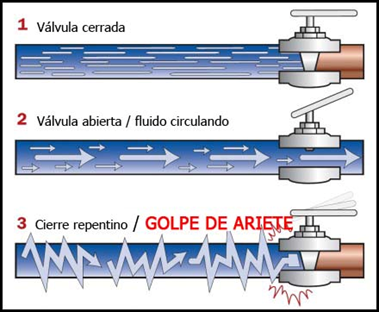
\includegraphics[width=0.6\linewidth]{fig1}
	\caption{Representación de un golpe de ariete en una tubería. (fuente: \url{http://www.empresasconstruccion.es/golpe-de-ariete-water-hammer-smagua-2014/}).}
	\label{fig:fig1}
\end{figure}
\end{center}
%******************************************

\section{Principio de operación de un sistema de protección contra golpe de ariete}
En la centrales hidroeléctricas y acueductos se instalan dispositivos de seguridad física de las tuberías de presión 
para limitar los efectos de sobrepresión, que se producen por encendido o para de la maquinaría hidráulica, como 
son las turbinas de generación o los equipos de bombeo.\bigskip

En las Figura \ref{fig:fig2} a \ref{fig:fig8} se muestran cámaras de oscilación a cielo abierto para controlar la sobrepresión y 
para el caso de tuberías de pequeño diámetro en la Figura \ref{fig:fig9} y Figura \ref{fig:fig10} se muestran configuraciones de las 
válvulas de no retorno, que producen cambios en la presión por efecto del paro de equipos de bombeos.
\begin{figure}[H]
	\centering
	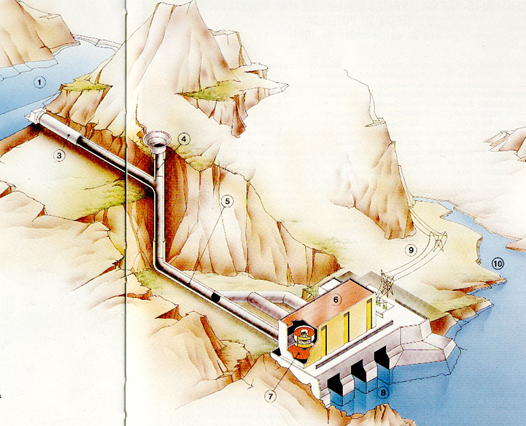
\includegraphics[width=.65\linewidth]{fig2}
	\caption{Esquema de la tubería de carga de una Central Hidroeléctrica.}
	\label{fig:fig2}
\end{figure}

\begin{figure}[H]
	\centering
	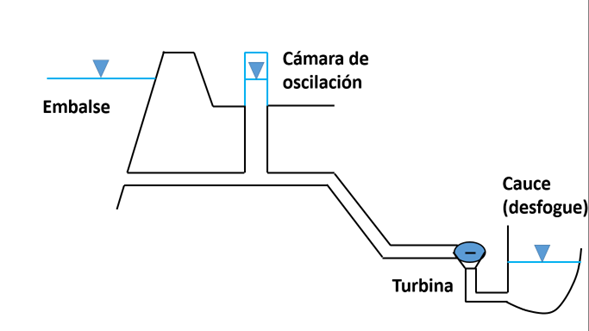
\includegraphics[width=0.65\linewidth]{fig3}
	\caption{Esquema de ubicación de una cámara de oscilación en una Central Hidroeléctrica (elaboración propia).}
	\label{fig:fig3}
\end{figure}

\newpage
\vspace*{2cm}
\begin{figure}[H]
	\centering
	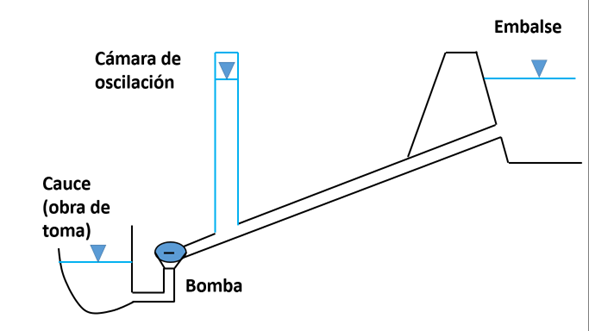
\includegraphics[width=0.65\linewidth]{fig4}
	\caption{Esquema de ubicación de la cámara de oscilación en una estación de bombeo (elaboración propia).}
	\label{fig:fig4}
\end{figure}
\vspace*{2cm}
\begin{figure}[H]
	\centering
	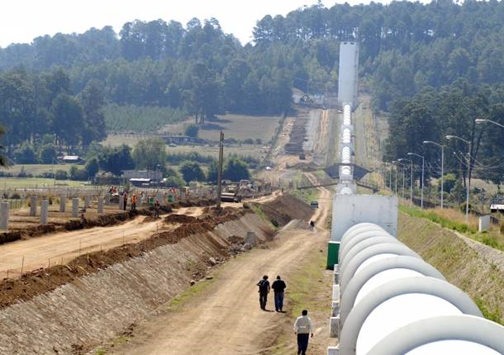
\includegraphics[width=.7\linewidth]{fig5}
	\caption{Línea de conducción del sistema Cutzamala y la cámara de oscilación (CONAGUA, 2011).}
	\label{fig:fig5}
\end{figure}

\newpage
\vspace*{2cm}
\begin{figure}[H]
	\centering
	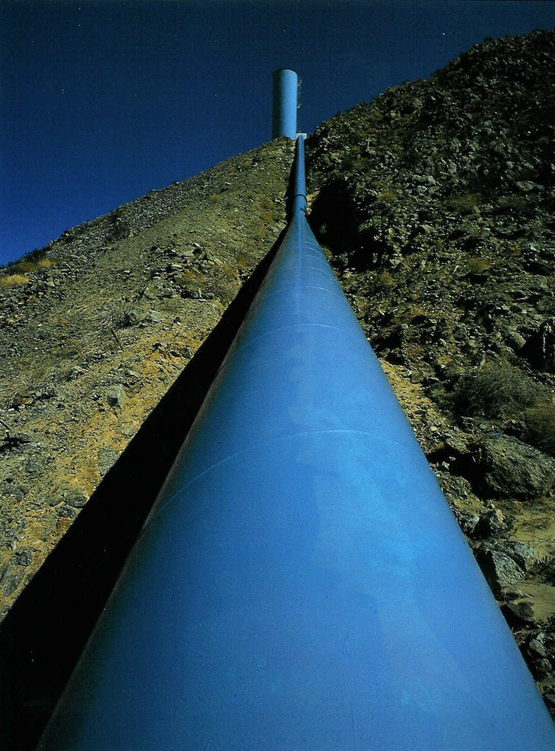
\includegraphics[width=0.8\linewidth]{fig6}
	\caption{Línea de conducción del acueducto Río Colorado – Mexicali (CONAGUA 2011).}
	\label{fig:fig6}
\end{figure}

\newpage
\vspace*{2cm}
\begin{figure}[H]
	\centering
	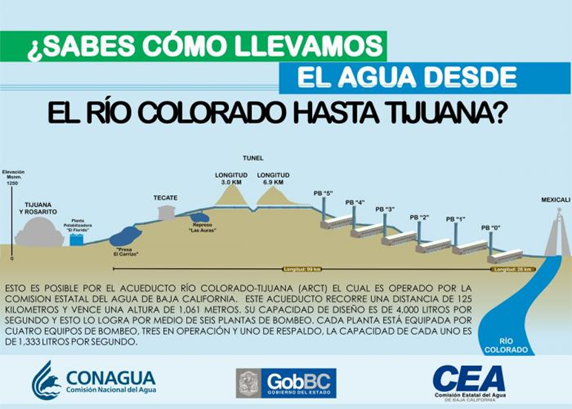
\includegraphics[width=0.7\linewidth]{fig7}
	\caption{Figura 2.7 Esquema de operación del acueducto de Mexicali-Tijuana).}
	\label{fig:fig7}
\end{figure}
\vspace*{1cm}
\begin{figure}[H]
	\centering
	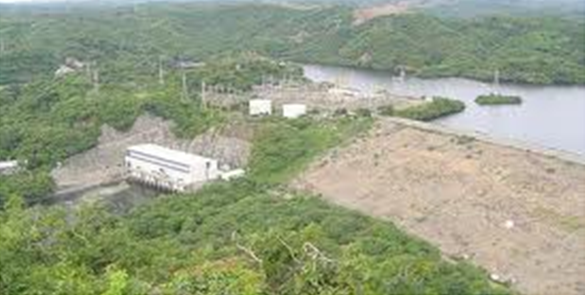
\includegraphics[width=.8\linewidth]{fig8}
	\caption{Central Hidroeléctrica José María Morelos (La Villita), (CFE, 2011).}
	\label{fig:fig8}
\end{figure}

\newpage
\vspace*{1cm}
\begin{figure}[H]
	\centering
	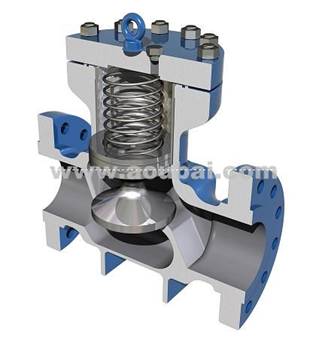
\includegraphics[width=0.5\linewidth]{fig9}
	\caption{Válvula de no retorno.}
	\label{fig:fig9}
\end{figure}
\vspace*{1cm}
\begin{figure}[H]
	\centering
	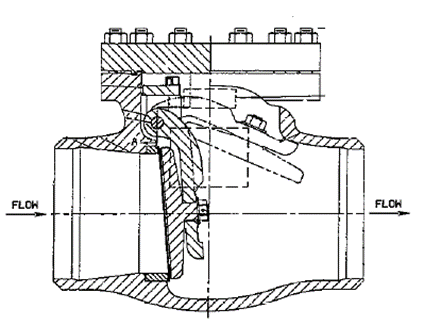
\includegraphics[width=.55\linewidth]{fig10}
	\caption{Válvula de no retorno (retención o Check).}
	\label{fig:fig10}
\end{figure}
\newpage

%******************************************
\section{Definiciones}
Como inicio en el estudio del golpe de ariete, primero se realizará una revisión a la historia del desarrolló 
del conocimiento de los transitorios hidráulicos en tuberías, así como el origen de las ecuaciones básicas del 
golpe de ariete provocado por el cierre instantáneo de una válvula y la representación de los cambios de la 
velocidad en el conducto. \bigskip

En este punto se presentarán las aproximaciones de los modelos matemáticos para describir la reflexión de ondas, 
inducidas por el cierre de la válvula agua abajo, y al final se hará una discusión de la causa de los fenómenos transitorios.\bigskip

\emph{Condición permanente y no permanente (transitorio).}\\
En campo de flujo en una tubería o canal algún fenómeno o magnitud no cambian en el tiempo se dice que se 
tiene una condición estacionaria o permanente, por ejemplo, para la velocidad, gasto y presión se dice:\bigskip

Si las condiciones de flujo, tal como la presión, velocidad o el caudal, en un punto de la conducción no cambian
 en el tiempo entonces \emph{el flujo está en una condición estacionaría o permanente}, por lo tanto:
\begin{equation}
	\frac{dV}{dt} = 0, \hspace{0.5cm} \frac{dQ}{dt} = 0, \hspace{0.5cm} \frac{dp}{dt} = 0 \hspace{0.5cm} \forall \ \ \ t
\end{equation}

En el caso contrario se tiene una condición \emph{transitoria (dicho de un fenómeno o magnitud que se encuentra entre 
dos regímenes estacionarios consecutivos durante un intervalo de tiempo)}.\bigskip

Nota: en forma específica todos los flujos cuando son turbulentos estos son no permanentes, ya que tienen o 
mantienen fluctuaciones temporales. Por ejemplo, esto se puede observar a la salida a gran velocidad en una 
tubería (Figura \ref{fig:fig11}). No obstante, lo anterior, se puede asumir que el promedio temporal, arroja un valor 
medio \emph{\underline{cuasi permanente}}. Para fines de este curso siempre se estará analizando el flujo medio o promediado y 
por lo tanto existen condiciones de flujo permanente para una condición de flujo turbulento (sic).\bigskip

\begin{figure}[H]
	\centering
	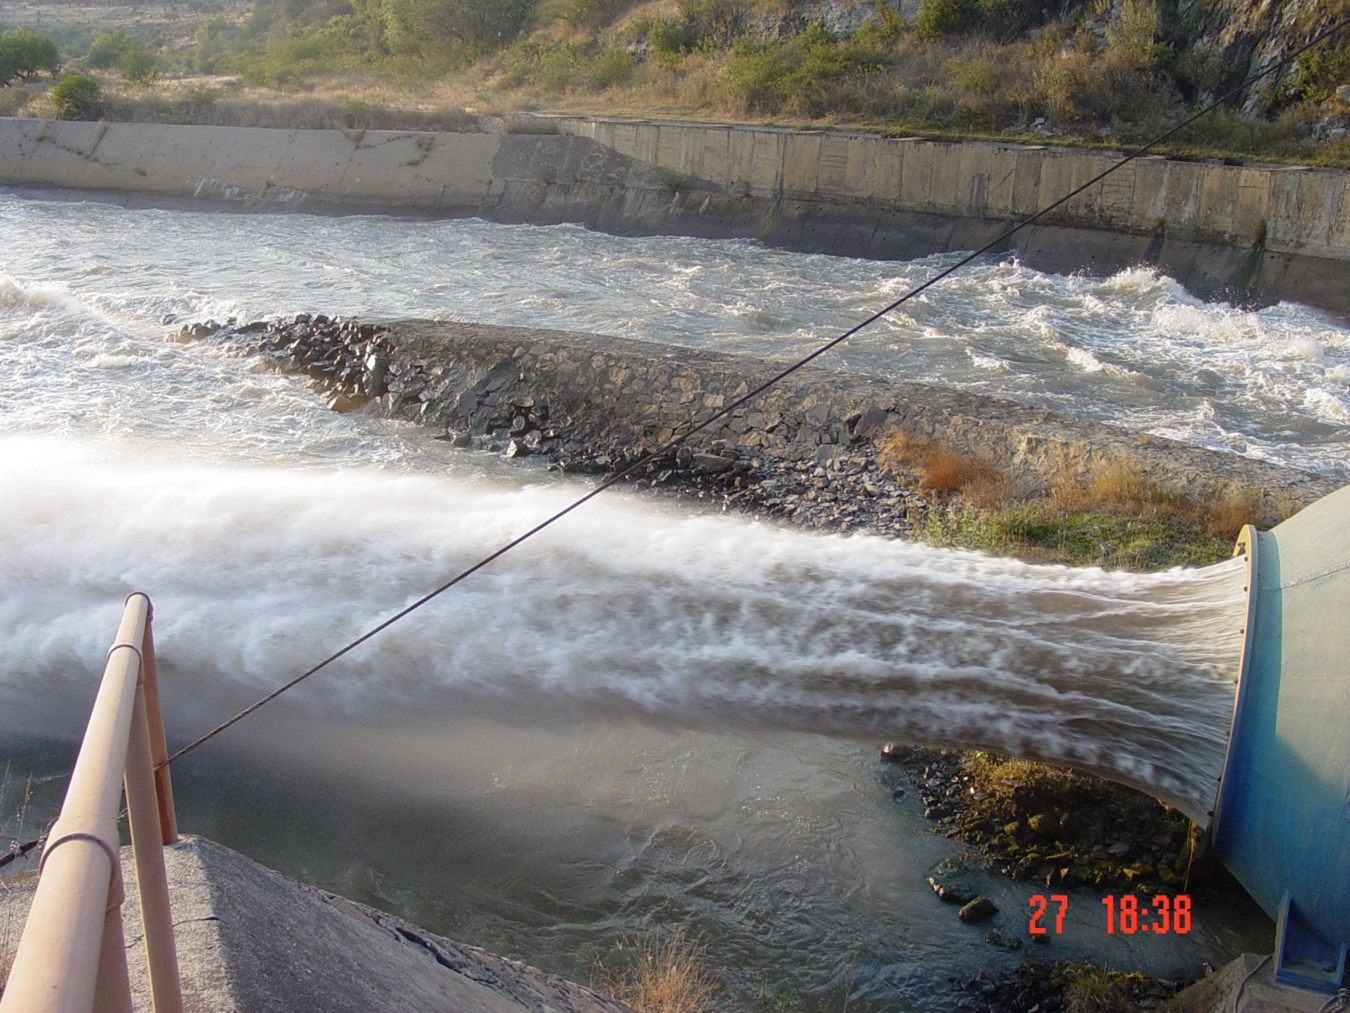
\includegraphics[width=.65\linewidth]{fig11}
	\caption{Descarga de la válvula de chorro convergente de obra de toma 1 de la presa Solís, Guanajuato, (Archivo, Ariosto Aguilar, 2004).}
	\label{fig:fig11}
\end{figure}

Entonces se dice que el flujo medio es aquel que se define como el promedio de una velocidad fluctuante para 
un intervalo conocido, por ejemplo, si la velocidad de una partícula se puede representar por el vector velocidad tal que:
\begin{equation}
\mathbf{q}(\mathbf{x},t)=u\mathbf{i}+v\mathbf{j}+w\mathbf{k}
\end{equation}

donde $\mathbf{q}(\mathbf{x},t)$, es el vector velocidad en un punto en el espacio y sus componentes por cada dirección son
 $(u,v,w)$ con su respectivo vector unitario por componente $(\mathbf{i}, \mathbf{j}, \mathbf{k})$; y su ubicación espacial
 se representa por el vector $\mathbf{x} \in \Omega(x, y, z)$, y la variación temporal se indica con la variable independiente $t$.\bigskip

La velocidad promediada para el sentido $x$ se puede expresar, como: 
\begin{equation}
	U = \frac{1}{T}\int_T {u(\mathbf{x}, t)dt}
\end{equation}

donde $U$, es la velocidad promedio; $T$, es el periodo de muestreo, y $u(\mathbf{x}, t)$ es la componente de la velocidad en el sentido $x$.\bigskip

\begin{figure}[H]
	\centering
	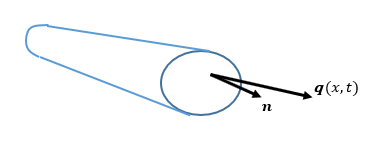
\includegraphics[width=.5\linewidth]{fig12}
	\caption{Vector velocidad sobre una sección transversal (elaboración propia).}
	\label{fig:fig12}
\end{figure}

En forma estricta, si el análisis es unidimensional, la velocidad media se representa de la forma siguiente:
\begin{equation}
	U = \frac{1}{T}\int_T \frac{1}{A}\int_S{\mathbf{q}(\mathbf{x}, t)} \bullet \mathbf{n} \ ds \ dt
\end{equation}

donde $S$, es la superficie normal al flujo; $\mathbf{n}$, es el vector normal a la superficie y $A$, el área transversal de la sección 
de la tubería o canal.\bigskip

\emph{Flujo transitorio}. Condición de flujo intermedio que se sucede entre dos condiciones de flujo permanente, en forma 
rigurosa la condición final del flujo permanente es nuevamente una condición cuasi permanente. Dentro del concepto de análisis 
de flujos medios si se tiene nuevamente una condición permanente.\bigskip

\emph{Flujo uniforme y no uniforme}. Este concepto define la evaluación espacial del cambio de la velocidad de un flujo para un 
tiempo específico, entonces:
\begin{equation}
\begin{aligned}
	\frac{dV}{dx} & = 0 \hspace{0.3cm} ;\hspace{0.3cm} \mbox{\emph{flujo uniforme}} \\
	\frac{dV}{dx} & \neq 0 \hspace{0.3cm} ;\hspace{0.3cm} \mbox{\emph{flujo no uniforme}}
\end{aligned}
\end{equation}

Por ejemplo, los perfiles de flujo en un cambio de pendiente de un canal, o los cambios que se tienen en las transiciones en tuberías y canales.\bigskip

\emph{Flujos periódicos u oscilatorios.} Esta definición se considera cuando el flujo varía en el tiempo y este se repite después de un intervalo fijo; 
a manera de ejemplo, se muestra la variación del flujo en el canal de marea a la entrada de la laguna de Bojórquez (Figura \ref{fig:fig13}). \bigskip

\begin{figure}[H]
	\centering
	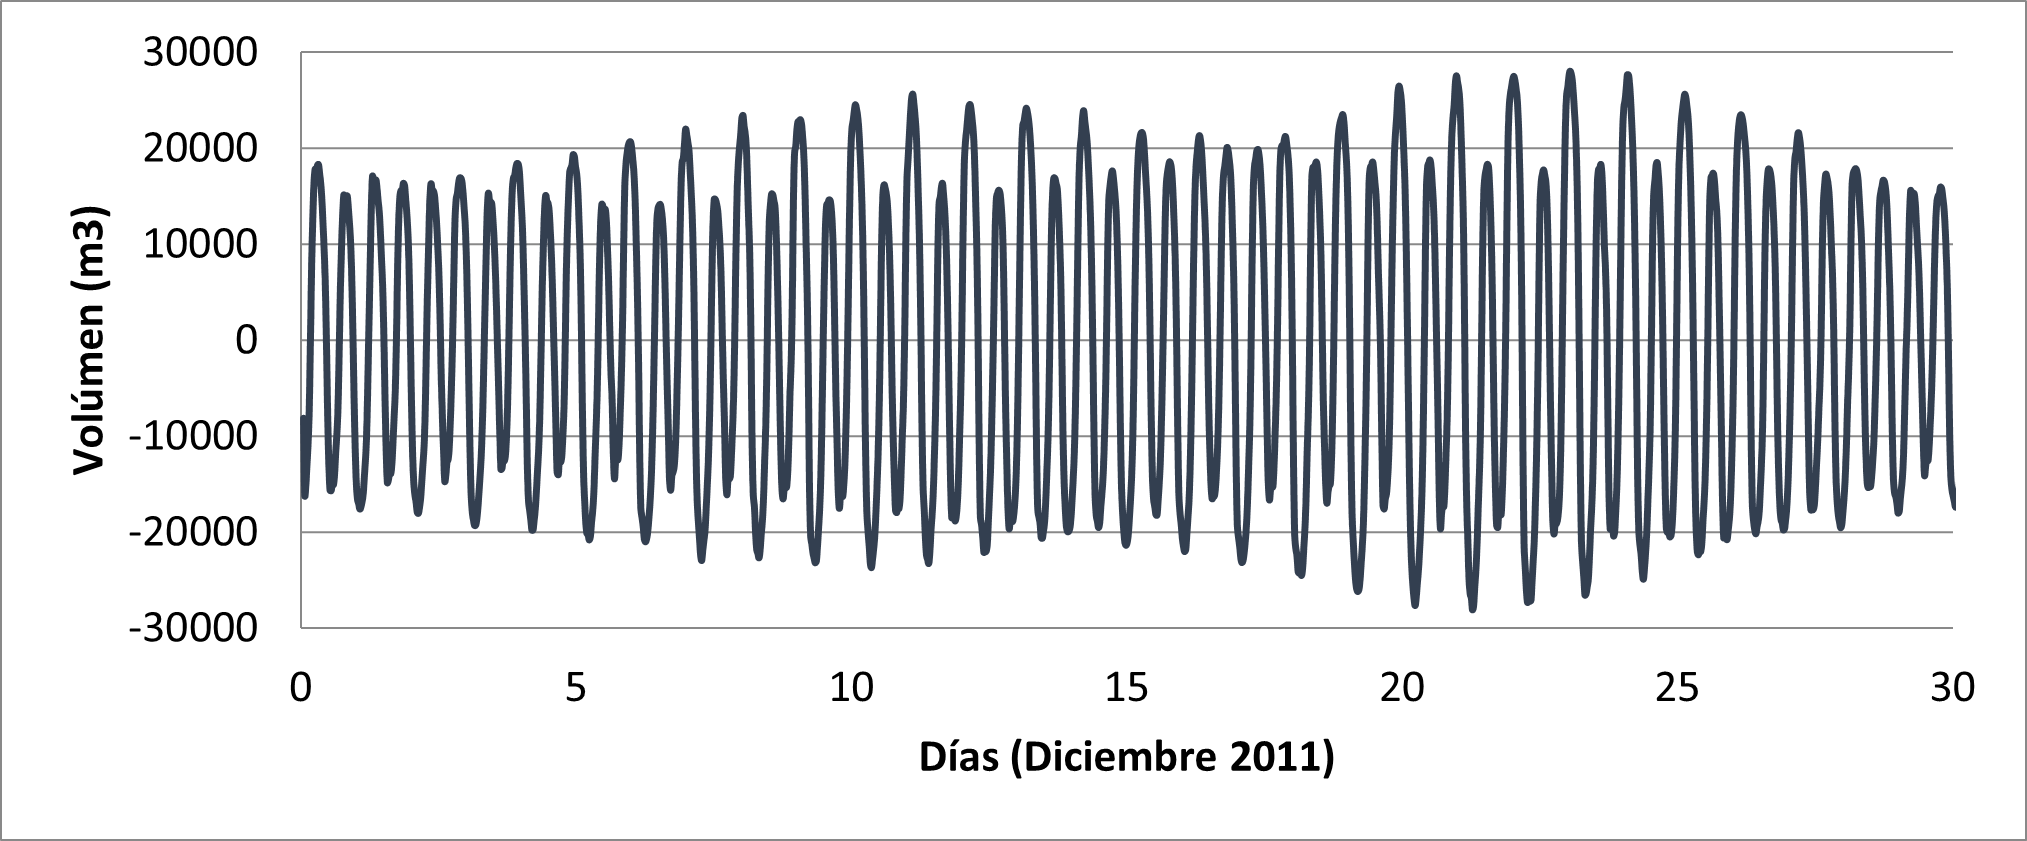
\includegraphics[width=.8\linewidth]{fig13}
	\caption{Caudal de entrada y salida a la laguna de Bojórquez, durante diciembre de 2011 (IMTA, 2011).}
	\label{fig:fig13}
\end{figure}

% +++++++
\begin{mdframed}[backgroundcolor=azulpastel]
\textbf{Antecedentes históricos del análisis de un flujo periódico en un medio continuo.}\\
En forma histórica Newton y Lagrange obtuvieron en forma teórica la velocidad del sonido en el aire, con un valor de 298.4 m/s y al compararlo con el valor
 experimental de 348 m/s, Laplace atribuyó esta diferencia a los errores provocados al desarrollar el protocolo experimental, mientras que Newton explicó 
que la diferencia se debía a presencia de partículas de aire y vapor en el medio de la propagación de la onda.\bigskip

Euler en su publicación De la Propagation du Son, ''Mémories de l’Acad, d. Wiss, Berlin (2014), desarrollo una teoría detalla de la propagación elástica de 
ondas y propuso la siguiente ecuación diferencial de propagación de onda:
\begin{equation}
	\frac{\partial^2 y}{\partial t^2}= a^2 \frac{\partial^2 y}{\partial x^2}
\end{equation}

donde $a^2=gh$; $x$, es la posición de equilibrio de una partícula; $y$, es el desplazamiento de la partícula, y $h$, es la altura de la columna de aire. En forma 
similar propuso como solución general la siguiente expresión:
\begin{equation}
	y = F(x+at) + f(x-at)
\end{equation} 

en la expresión anterior $F$ y $f$ son las ondas viajantes, con este modelo Euler intentó describir el flujo de la sangre en las arterias, pero no tuvo el éxito esperado; 
no obstante, lo anterior, esta ecuación continúa siendo un modelo matemático para describir el comportamiento de una onda en un medio continuo.
\begin{mdframed}[backgroundcolor=verdeclaro]
Representación de una función continua en serie de Fourier\\
Las funciones que tienen una característica cambio periódico son las trigonométricas y la longitud de onda y frecuencia se pueden establecer de la siguiente forma:
\begin{equation*}
F(x, t) = Ae^{i(kx-\omega t)}
\end{equation*}

donde $k$ es la longitud de onda y $\omega$ la frecuencia, en forma estricta es posible tener diferentes longitudes de onda y estas también sería solución del problema, 
por lo tanto, la solución general es:
\begin{equation*}
F(x, t) = A_n \sum_{n=0}^\infty e^{i(k_nx-\omega(k_n)t)}
\end{equation*}
La serie anterior presenta la superposición lineal ondas de diferente longitud y frecuencias.\bigskip

\centering
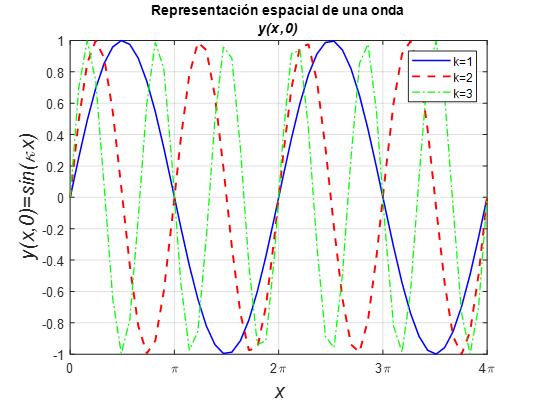
\includegraphics[width=0.8\linewidth]{f01}
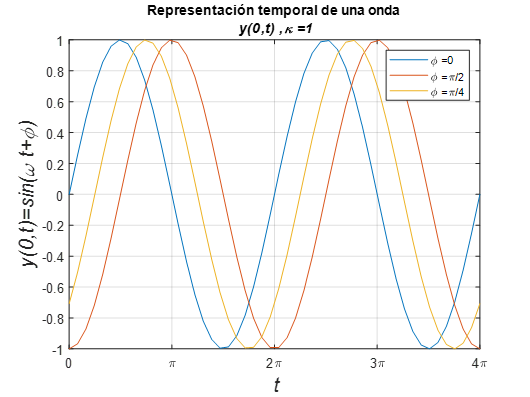
\includegraphics[width=0.8\linewidth]{f02}
\end{mdframed}

\begin{mdframed}[backgroundcolor=verdeclaro]
\centering
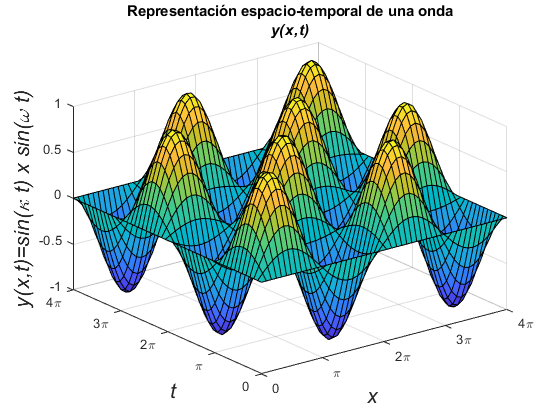
\includegraphics[width=0.8\linewidth]{f03}
\end{mdframed}

Posteriormente Lagrange, analizó los fluidos compresibles y no compresibles, y para analizarlo propuso el concepto de velocidad potencial y generó la expresión para 
identificar la celeridad de onda para un canal y se expresa con la siguiente relación:
\begin{equation}
	c = \sqrt{gd}
\end{equation}
donde $d$, es el tirante del canal y $g$ es la aceleración de la gravedad.\bigskip

En un trabajo posterior Helmholtz fue el primero en describir que las ondas de velocidad del agua por efecto de la presión, confinadas en una tubería son mayores a 
las que se tienen en agua no confinada. Según Chaudry (1979) este concepto es correcto ya que está diferencia es debida a la elasticidad de la pared de las tuberías.\bigskip

En 1869, Riemann en su publicación Partielle Differentialgleichungen (Chaudry 1979) desarrolló y aplicó una ecuación en tres dimensiones de movimiento y una forma 
simplificada unidimensional, conocida como la teoría básica de cuerdas vibrantes y velocidad de ondas.\bigskip

En 1897, Joukowski realizó experimentos extensivos en tuberías y basado en estos estudios experimentales y teóricos desarrolló el análisis básico del golpe de ariete. 
Este modelo considera una fórmula para la velocidad de la onda, tomando en cuenta los cambios elásticos de la columna de agua y la pared de la tubería. Además, 
construyó una relación entre la reducción de la velocidad y el incremento de la presión, y utiliza dos principios de la física, la ecuación de la conservación de la 
energía y la de continuidad.\bigskip

Posteriormente, Allievi en 1902, desarrolla una teoría general del golpe de ariete e introduce los siguientes parámetros adimensionales:
\begin{align}
	\rho & = \frac{aV_o}{2gH_o}\\
	\theta & = \frac{aT_c}{2L}
\end{align}

donde $a$, es la velocidad de onda del golpe de ariete; $V_o$, velocidad del agua a condición permanente; $L$, longitud de la tubería; $T_c$, tiempo de cierre; $\rho$, es 
la mitad de la relación de la energía cinética del fluido de la energía potencial almacenada en el fluido y en las paredes del tubo a una carga de presión $H_o$ y 
$\theta_o$, es la característica de cierre de la válvula.
\end{mdframed}
% ++++++

\emph{Propagación de onda y reflexiones en una tubería simple}\\
Sea una tubería, como la mostrada en la lámina 4.4, conectada a un almacenamiento con una operación a flujo permanente para $t=0$ y la válvula es cerrada rápidamente. 
Considerando un sistema sin fricción, la carga de presión a todo lo largo de la tubería será $H_o$ (en este análisis se considerará la distancia como $x$ y la velocidad 
$V$ como positiva en el sentido hacia aguas abajo).
La secuencia de eventos que se suceden después del cierre de la válvula se divide en cuatro y son:
\begin{enumerate}[I.]
	\item $0<t\le\frac{L}{a}$ (Figura \ref{fig:fig14}a y \ref{fig:fig14}b) Tan pronto como la válvula es cerrada, la velocidad del flujo en la válvula se reduce a cero, lo cual produce que la 
	presión se elevé a $\Delta H = + \frac{a}{g}V_o$. Esto es debido a que la presión en la tubería sube, la tubería se expande (en la Figura \ref{fig:fig14}b se muestra este efecto de 
	expansión con línea punteada), el fluido es comprimido con el consecuente aumento de la densidad y la presión positiva viaja hacia el embalse. Detrás de esta onda la 
	velocidad es cero y toda la energía cinética se convierte en energía elástica. Si a es la velocidad de la onda del golpe de ariete y $L$ es la longitud de la tubería, 
	entonces en el tiempo $t=L/a$, a lo largo de toda la tubería, el tubo se expande y el flujo es cero y la presión es $H_o+\Delta H$.
	\item $\frac{L}{a} < t \le 2\frac{L}{a}$ (Figura \ref{fig:fig14}c y \ref{fig:fig14}d) Como el nivel del almacenamiento es constante, las condiciones son inestables en el almacenamiento cuando 
	la onda llega, porque la presión en la sección adjunto del almacenamiento es $H_o$, mientras que la presión en la tubería es $H_o+\Delta H$. Debido a esta diferencial de presiones, 
	el fluido empieza a moverse desde la tubería hace el almacenamiento con una velocidad $-V_o$, entonces la velocidad cambia de 0 a $-V_o$ lo cual produce que la presión decrezca 
	de $H_o+\Delta H$ a $H_o$. En otras palabras, una onda negativa viaja desde la válvula por la onda presión hasta que se tiene la carga $H_o$. Para $t = 2L/a$ la carga de presión en 
	la tubería es $H_o$ y el fluido es $-V_o$.
	\item $2\frac{L}{a} < t \le 3\frac{L}{a}$ (Figura \ref{fig:fig14}e y \ref{fig:fig15}f) Debido a que la válvula está cerrada, la velocidad negativa no se puede mantener en la válvula. 
	Por este motivo, la velocidad se cambia instantáneamente de $-V_o$ a 0, y debido a esto la presión se reduce a $H_o-\Delta H$ y una onda negativa se propaga en la dirección 
	hacia aguas arriba. Detrás de esta onda, la presión es $H_o-\Delta H$ y el fluido es cero. Para el tiempo $t=3L/a$, la carga de presión en toda la tubería es $H_o-\Delta H$ y la 
	velocidad es cero.
	\item	$3\frac{L}{a} <t \le 4\frac{L}{a}$ (Figura \ref{fig:fig15}g y \ref{fig:fig15}h) Tan pronto como la velocidad negativa alcanza el embalse, condición de desbalance se vuelve a generar. Ahora la 
	presión es mayor en el lado del embalse que en la tubería. Entonces el fluido empieza a viajar desde el embalse hacia la válvula con una velocidad $V_o$ y una carga de presión de 
	almacenamiento $H_o$. Para el tiempo $t=4L/a$, la carga de presión es $H_o$ y la velocidad del flujo es $V_o$, entonces se tienen las mismas condiciones iniciales de flujo para 
	la condición permanente.
\end{enumerate}
Los eventos de cambio de presión y velocidad se muestran en la Figura \ref{fig:fig16} y son los que suceden cuando no hay fricción, en el caso real los eventos de cambio de presión se muestran 
en la Figura \ref{fig:fig17}.

\begin{figure}[H]
	\centering
	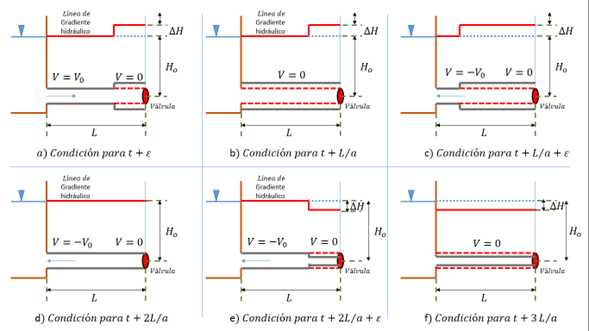
\includegraphics[width=0.90\linewidth]{fig14}
	\caption{Propagación de una onda de presión causada por el cierre instantáneo de una válvula (elaboración propia).}
	\label{fig:fig14}
\end{figure}

\begin{figure}[H]
	\centering
	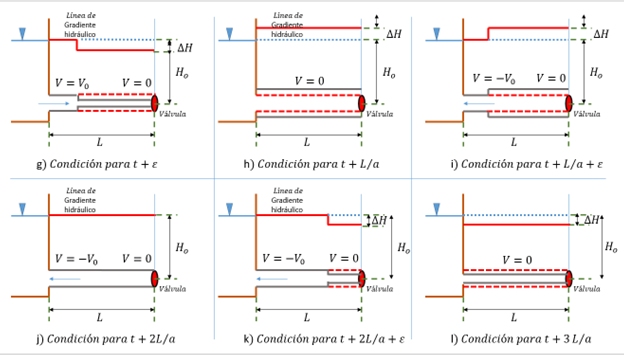
\includegraphics[width=0.90\linewidth]{fig15}
	\caption{Propagación de una onda de presión causada por el cierre instantáneo de una válvula (elaboración propia).}
	\label{fig:fig15}
\end{figure}
\begin{figure}[H]
	\centering
	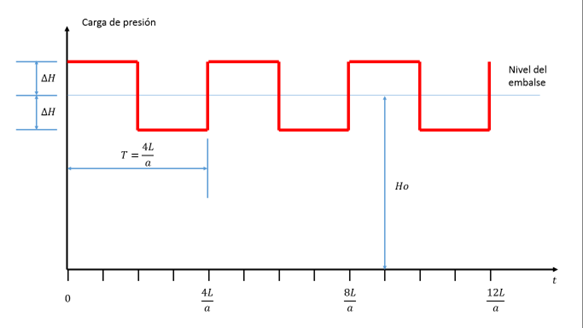
\includegraphics[width=0.90\linewidth]{fig16}
	\caption{Secuencia de eventos para el cierre de la válvula sin fricción (elaboración propia).}
	\label{fig:fig16}
\end{figure}
\begin{figure}[H]
	\centering
	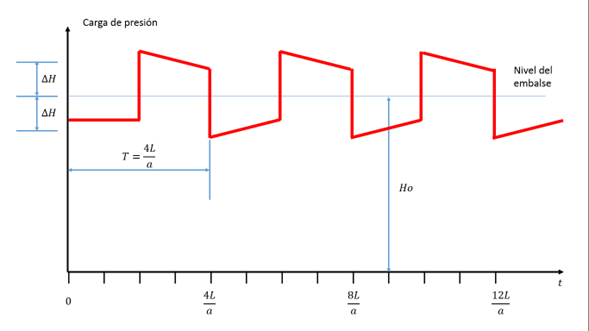
\includegraphics[width=0.90\linewidth]{fig17}
	\caption{Secuencia de eventos para el cierre de la válvula con fricción (elaboración propia).}
	\label{fig:fig17}
\end{figure}
\clearpage
\newpage
\mbox{}

%******************************************
\section{Origen de los transitorios en conductos cerrados}
Tal como se definió anteriormente, los flujos transitorios se originan entre dos eventos de flujo permanente y entonces se dice que la condición permanente es perturbada. Estos cambios o 
perturbaciones pueden ser planeados o incidentales y en la puesta en operación de un equipo se tienen que dejar los procedimientos o equipos para que el sistema no presente fallas por los 
cambios que se suceden durante el flujo transitorio.\bigskip

Los casos más comunes de flujo transitorio son:
\begin{enumerate}[a.]
	\item Apertura, cerrado o no retorno originado por válvulas en la tubería.
	\item Inicio o paro de los equipos de bombeo.
	\item Inicio o paro de turbinas hidráulicas.
	\item Cambios súbitos en el flujo de un canal, provocados por una compuerta.
	\item Fallo o colapso de una presa.
	\item Incrementos súbitos de flujo en un río por efecto de una avenida o creciente.
\end{enumerate}

%******************************************
\section{Ecuaciones fundamentales}
El flujo no permanente en un conducto cerrado se describe con las ecuaciones de continuidad y de cantidad de movimiento.
Consideraciones:
\begin{itemize}
	\item El flujo es unidimensional y la distribución de las velocidades sobre la sección transversal del conducto es uniforme.
	\item Las paredes del tubo y el fluido son linealmente elásticas. Lo anterior se aplica en la mayoría de los conductos como son: el metal, concreto, madera, plásticos o túneles 
	no revestidos en rocas.
	\item Las fórmulas para calcular las pérdidas de fricción en condición permanente en conductos se consideran válidas durante el análisis transitorio (por ejemplo: Darcy-Weisbach).
\end{itemize}
	 
Nota: esta consideración siempre es controversial, pero en últimas fechas con el uso de los modelos de Dinámica de Fluidos Computacional se ha demostrado que su aplicación es válida, 
para el tipo de estudio de flujo transitorio.

\subsection{Ecuación de cantidad de movimiento}
En la Figura \ref{fig:fig18} se describe un esquema del flujo en una tubería, y la variable espacial $x$ en el sentido de la tubería, y dado que se tiene una condición no permanente la variable $t$, 
es el tiempo.\bigskip

\begin{figure}[H]
	\centering
	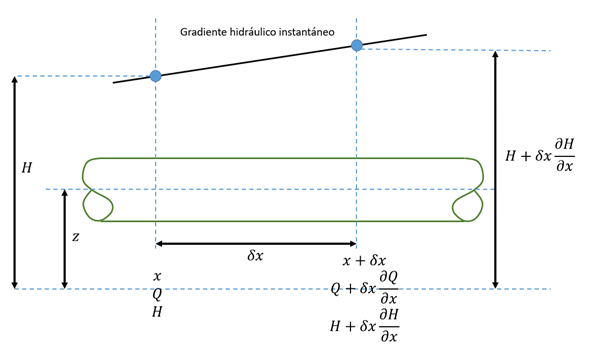
\includegraphics[width=0.7\linewidth]{fig18}
	\caption{Variación del gradiente hidráulico instantáneo (elaboración propia).}
	\label{fig:fig18}
\end{figure}

Para evaluar los cambios de las variables dependientes $Q(x, t)$, gasto; $V(x,t)$,  velocidad y $H(x,t)$, carga de presión, se considera una aproximación de primer orden sobre un 
incremento en la distancia $\delta x$, entonces se dice:\bigskip

Para la condición espacial x se tienen las variables $Q(x,t)$, $V(x,t)$  y $H(x,t)$ , y para $x+\delta x$ se tienen la condición $Q(x+\delta x,t)$, $V(x+\delta x,t)$  y $H(x+\delta x,t)$, 
aplicando una expansión en serie de Taylor, entonces:
\begin{align}
	Q(x+\delta x,t) & = Q(x,t)+\delta x \frac{\partial Q}{\partial x} + \cdots\\
	V(x+\delta x,t) & = V(x,t)+\delta x \frac{\partial V}{\partial x} + \cdots\\
	H(x+\delta x,t) & = H(x,t)+\delta x \frac{\partial H}{\partial x} + \cdots
\end{align}

\begin{mdframed}[backgroundcolor=verdeclaro]
\textbf{Descripción del espacio de solución y su relación con las variables del fenómeno}\\
En esta parte el espacio de solución se define como:
\begin{equation*}
	\Omega(x,t) \in \mathbb{R}^2
\end{equation*}

donde $x$ es la coordenada espacial y $t$ el tiempo, como variables independientes.\bigskip

Para los transitorios en tuberías y canales el espacio de solución se delimita a la longitud de la tubería o canal ($L$) y al tiempo de análisis del flujo transitorio ($T$), entonces se dice:
\begin{equation*}
(x,t) \in \Omega =[0,L]\times[0,T]
\end{equation*}

Las variables dependientes son gasto $Q(x,t)$, velocidad $V(x,t)$ y carga hidráulica $H(x,t)$, entonces se dice:
\begin{equation*}
Q,V,H:\Omega
\end{equation*}

La relación anterior se describe en la Figura siguiente, en donde se tiene el espacio de solución $\Omega$, acotado por los ejes espacio temporal y para cada valor es este espacio se tiene 
un correspondiente valor de la variable dependiente.
\centering
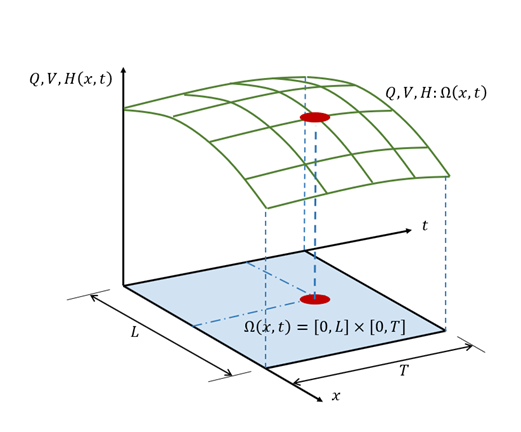
\includegraphics[width=0.7\linewidth]{f04}
\end{mdframed}

Las fuerzas actuantes sobre el volumen son $F_1$, $F_2$ y $S$, en donde $F_1$, $F_2$ son la fuerza de presión y $S$ es los efectos de las fuerzas de fricción (Figura \ref{fig:fig19}).\bigskip

\begin{figure}[H]
	\centering
	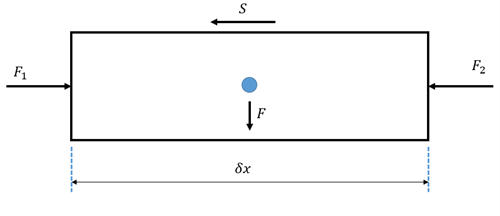
\includegraphics[width=0.7\linewidth]{fig19}
	\caption{Diagrama de cuerpo libre de las fuerzas que actúan sobre un volumen de fluido (elaboración propia).}
	\label{fig:fig19}
\end{figure}

Para evaluar las fuerzas que actúan en el volumen se consideran las presiones en las caras externas del volumen ($\rho gzA$) y la fuerza de fricción, a un nivel referencia arbitrario $z$, 
entonces se tiene:
\begin{align}
	F_1 & = \rho g A (H-z) \label{eq:f1}\\
	F_2 & = \rho g A \left( H + \delta x \frac{\partial H}{\partial x} -z \right) \label{eq:f2}\\
	S &= \rho g A f \frac{\partial x}{D}\frac{V^2}{2g} \label{eq:S}
\end{align}
donde $f$ es el factor de fricción de Darcy.\bigskip

La fuerza resultante coplanar se tiene para:
\begin{equation}
	 F=F_1-F_2-S
\label{eq:F}
\end{equation}

Entonces, sustituyendo las ecuaciones \ref{eq:f1}, \ref{eq:f2} y \ref{eq:S} en \ref{eq:F} y desarrollando se tienen la suma de fuerzas actuantes:
\begin{equation}
	\begin{aligned}
		F &=\rho g A(H-z) -\rho g A \left(H + \delta x \frac{\partial H}{\partial x} -z \right) -\rho A f \frac{\delta x}{D} \frac{V^2}{2} \\
				F & =\rho g A(H-z)-\rho g A(H-z)-\rho gA\delta x\frac{\partial H}{\partial x}-\rho Af\frac{\delta x}{D}\frac{V^2}{2}\\
		F & =-\rho A\delta x\left(g\frac{\partial H}{\partial x}+\frac{f}{D}\frac{V^2}{2}\right)
	\end{aligned}
	\label{eq:FF}
\end{equation}

Para evaluar los cambios en la aceleración sobre la masa del volumen de control, por efectos de las fuerzas actuantes se aplica la segunda la segunda Ley de Newton de forma que:
\begin{equation}
	f = m\frac{dV}{dt}
\label{eq:2da}
\end{equation}

En este caso la masa del volumen en análisis se considera como $m=\rho A\delta x$, sustituyendo en la ecuación \ref{eq:2da} y además la fuerza evaluadas en \ref{eq:FF}, se tiene:
\begin{equation*}
	-\rho A \delta x \left( g\frac{\partial H}{\partial x} + \frac{f}{D} \frac{V^2}{2} \right) = \rho A \delta x \frac{dV}{dt}
\end{equation*}

O también:
\begin{equation}
	\frac{dV}{dt} = -g \frac{\partial H}{\partial x} - \frac{f V^2}{2D}
\end{equation}

La diferencial total para el cambio de velocidad se obtiene aplicando la ley de la cadena para una función de varias variables:
\begin{equation*}
dV(x,t) = \frac{\partial V}{\partial t} dt + \frac{\partial V}{\partial x} dx
\end{equation*}

Considerando la variación temporal sobre la velocidad, entonces la ecuación anterior se escribe como:
\begin{equation}
\frac{dV}{dt}=\frac{\partial V}{\partial t}+\frac{\partial V}{\partial x}\frac{dx}{dt}
\label{eq:dvdt}
\end{equation}

En la expresión \ref{eq:dvdt}, el término $V=\frac{dx}{dt}$ indica el transporte cinemático de las ondas o advección, entonces:
\begin{equation}
	\frac{dV}{dt}=\frac{\partial V}{\partial t}+V\frac{\partial V}{\partial x}
\label{eq:dvdt2}
\end{equation}

Sustituyendo \ref{eq:dvdt2} en \ref{eq:dvdt}:
\begin{equation}
\frac{\partial V}{\partial t}+V\frac{\partial V}{\partial x}+g\frac{\partial H}{\partial x}+\frac{fV^2}{2D}=0
\label{eq:pvpt}
\end{equation}

En las Figuras \ref{fig:fig16} y \ref{fig:fig17} se observa que el flujo puede cambiar de dirección, entonces para evaluar este cambio de 
dirección, en función del análisis de la cantidad de movimiento (Figura 2.18), entonces el término de la fricción en la ecuación 
\ref{eq:pvpt} se puede evaluar como:
\begin{equation}
\frac{\partial V}{\partial t}+V\frac{\partial V}{\partial x}+g\frac{\partial H}{\partial x}+\frac{f\left|V\right|V}{2D}=0
\label{eq:pvpt2}
\end{equation}

Ahora, expresando la ecuación \ref{eq:pvpt2} en términos del gasto se tiene:
\begin{equation*}
\frac{\partial Q}{\partial t}\frac{1}{A}+\frac{Q}{A^2}\frac{\partial Q}{\partial x}+g\frac{\partial H}{\partial x}+\frac{1}{A^2}\frac{f\left|Q\right|Q}{2D}=0
\end{equation*}

o también:
\begin{equation}
\frac{\partial Q}{\partial t}+\frac{Q}{A}\frac{\partial Q}{\partial x}+gA\frac{\partial H}{\partial x}+\frac{1}{A}\frac{f\left|Q\right|Q}{2D}=0
\label{eq:continuidad}
\end{equation}

\subsection{Ecuación de conservación de masa}
Del volumen diferencial en análisis (Figura 2.18)  se considerará los cambios en la masa, realizando un balance entre las entradas y salidas, 
entonces:
\begin{align}
	\forall_{entrada} &= V\frac{\pi D^2}{4}\delta t \\
	\forall_{salida} &=\left(V+\frac{\partial V}{\partial x}\delta x\right)\frac{\pi D^2}{4}\delta t
\end{align}
Aplicando el principio de conservación de masa, se dice que las expansiones o contracciones de la vena líquida sometida por el efecto del golpe de ariete 
son:
\begin{align*}
	&\delta\forall = \forall_{entrada}-\forall_{salida}\\
	&\delta\forall = V\frac{\pi D^2}{4}\delta t-\left(V+\frac{\partial V}{\partial x}\delta x\right)\frac{\pi D^2}{4}\delta
\end{align*}

O también:
\begin{equation}
	\delta\forall=-\frac{\partial V}{\partial x}\delta x\frac{\pi D^2}{4}\delta t
\label{eq:todoA}
\end{equation}

\emph{Modelo para evaluar los efectos elásticos en la tubería.}\\ 
Los cambios en la presión $\delta p$, que suceden para el intervalo $\delta t$ son $\left (\dfrac{\partial p}{\partial t}\right )\delta t$. Este cambio en la presión 
produce que las paredes del conducto se expandan o se contraigan en forma radial y producen que la longitud del elemento del fluido sea incrementado o 
disminuido, condición de un fluido compresible (ver Figura \ref{fig:fig20})\bigskip

\begin{figure}[H]
	\centering
	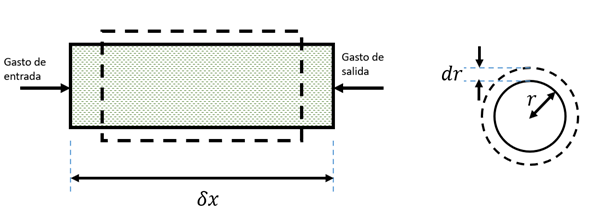
\includegraphics[width=0.7\linewidth]{figuras/fig20}
	\caption{Variables para la evaluar la elasticidad de la tubería (elaboración propia).}
	\label{fig:fig20}
\end{figure}

\underline{Cambios de volumen en la tubería.}
Entonces para los efectos de los cambios en la presión, en primera instancia consideramos estos efectos sobre el volumen, $\forall V$, se relacionan 
a la contracción o ampliación radial de la tubería. El esfuerzo radial o de aro, $\sigma$ en un conducto debido a la presión $p$ se indica con la ecuación siguiente:
\begin{equation}
 \sigma= \frac{pr}{e}
\label{eq:sigma}
\end{equation}

donde $e$, es el espesor de la tubería. Para evaluar los cambios en el esfuerzo radial $\delta\sigma$, se considera que estos están relacionados con 
el cambio de presión $\delta p$, entonces la ecuación \ref{eq:sigma} se escribe como:
\begin{equation}
	\delta\sigma=\delta p\frac{r}{e}=\frac{\partial p}{\partial t}\delta t\frac{r}{e}
\label{eq:psigma}
\end{equation}

Dado que el radio, $r$, se incrementa para $r+\delta r$, el cambio en la tensión se tiene para:
\begin{equation}
	\delta\epsilon=\frac{\delta r}{r}
\label{eq:epsilon}
\end{equation}

Si las paredes del tubo se consideran linealmente elásticas, entonces:
\begin{equation}
	E=\frac{\delta\sigma}{\delta\epsilon}
\label{eq:young}
\end{equation}

donde $E$, es el módulo de elasticidad de Young. Sustituyendo las expresiones para $\delta\sigma$ y $\delta\epsilon$, ecuaciones \ref{eq:psigma} y 
\ref{eq:epsilon}, en la ecuación \ref{eq:young} se tiene:
\begin{equation*}
	E=\dfrac{\dfrac{\partial p}{\partial t} \delta t \dfrac{r}{e}}{\dfrac{\delta r}{r}}
\end{equation*}

O también:
\begin{equation}
	\delta r=\frac{\partial p}{\partial t}\frac{r^2}{eE}\delta t
\label{eq:sr}
\end{equation}

El cambio de volumen de elemento diferencial, sometido a una expansión o contracción radial en un conducto se puede expresar como:
\begin{equation}
	\delta\forall_r=2\pi r\ \delta x\ \delta r
	\label{eq:da}
\end{equation}

Sustituyendo la evaluación de $\delta r$, ecuación \ref{eq:sr} en \ref{eq:da} se tiene:
\begin{equation}
	\delta\forall_r=2\pi r\ \delta x\ \frac{\partial p}{\partial t}\frac{r^2}{eE}\delta t
	\label{eq:dar}
\end{equation}

\emph{Modelo para evaluar los cambios en el volumen del fluido}\\
En este punto se generará una expresión para evaluar el cambio del volumen derivado de la compresibilidad del fluido $\delta\forall_c$, entonces si el volumen inicial del fluido se tiene:
\begin{equation}
	\forall=\pi r^2\delta x
	\label{eq:kel}
\end{equation}

El módulo de elasticidad de un fluido K se define como (Streeter y Wylie, 1976):
\begin{equation}
	K=-\frac{\delta p}{\dfrac{\delta\forall_c}{\forall}}
	\label{eq:k1}
\end{equation}

Sustituyendo \ref{eq:kel} en\ref{eq:k1} y considerando que $\delta p(t)=\dfrac{\partial p}{\partial t}\delta t$, entonces la ecuación anterior se evalúa como:
\begin{align*}
	\frac{\delta\forall_c}{\forall} &=-\frac{\delta p}{K}\\
	\frac{\delta\forall_c}{\pi r^2\delta x} &=-\frac{\delta p}{K}=-\frac{\partial p}{\partial t}\frac{\delta t}{K}
\end{align*}

Finalmente,
\begin{equation}
	\delta\forall_c=-\frac{\partial p}{\partial t}\frac{\delta t}{K}\pi r^2\delta x
	\label{eq:dda}
\end{equation}

Considerando que la densidad del fluido permanece constante, entonces la ecuación de conservación de masa se puede evaluar como:
\begin{equation}
	\delta\forall+\delta\forall_c=\sigma\forall_r
	\label{eq:daa}
\end{equation}

Entonces substituyendo las ecuaciones \ref{eq:todoA}, \ref{eq:dar}  y \ref{eq:dda} en \ref{eq:daa}:
\begin{equation*}
	-\frac{\partial V}{\partial x}\delta x\frac{\pi D^2}{4}\delta t-\frac{\partial p}{\partial t}\frac{\delta t}{K}\pi r^2\delta x=2\pi r\ \delta x\ \frac{\partial p}{\partial t}\frac{r^2}{eE}\delta t
\end{equation*}

Desarrollando:
\begin{align*}
	-\frac{\partial V}{\partial x}\frac{D^2}{4}-\frac{\partial p}{\partial t}\frac{1}{K}r^2 &=2r\ \ \frac{\partial p}{\partial t}\frac{r^2}{eE}\\
	-\frac{\partial V}{\partial x}\frac{{4r}^2}{4}-\frac{\partial p}{\partial t}\frac{1}{K}r^2 &=2r\ \ \frac{\partial p}{\partial t}\frac{r^2}{eE}
\end{align*}

\begin{equation*}
	\frac{\partial V}{\partial x}+\frac{\partial p}{\partial t}\frac{1}{K}+\ \ \frac{\partial p}{\partial t}\frac{2r}{eE}=0
\end{equation*}

Factorizando,
\begin{equation}
	\frac{\partial V}{\partial x}+\frac{\partial p}{\partial t}\left(\frac{2r}{eE}+\frac{1}{K}\right)= 0
	\label{eq:ec3}
\end{equation}

En este caso se tiene que $\rho$, es la densidad del fluido y la presión se puede evaluar bajo la condición hidrostática tal que $p=\rho gH$ y además, considerando la evaluación para el gasto, tal que $Q(x,t)=V\left(x,t\right)A$, entonces la ecuación \ref{eq:ec3}, se puede expresar, como:
\begin{equation*}
	A\frac{\partial Q}{\partial x}+\rho g\frac{\partial H}{\partial t}\left(\frac{2r}{eE}+\frac{1}{K}\right)=\ 0
\end{equation*}

Desarrollando,
\begin{align*}
	&\frac{\partial H}{\partial t}+\frac{1}{\rho gA}\frac{\partial Q}{\partial x}\left(\frac{D}{eE}+\frac{1}{K}\right)^{-1} = 0\\
	&\frac{\partial H}{\partial t}+\frac{1}{gA}\frac{\partial Q}{\partial x}\frac{K}{\rho\left(1+\dfrac{KD}{eE}\right)} = 0
\end{align*}

Finalmente, la ecuación de conservación de masa se expresa, como:
\begin{equation}
	\frac{\partial H}{\partial t}+\frac{a^2}{gA}\frac{\partial Q}{\partial x}=0
\end{equation}

donde
\begin{equation}
	a^2=\dfrac{K}{\rho\left[1+\dfrac{KD}{eE}\right]}
\end{equation}
El término $a$ se le conoce como la velocidad de propagación del golpe de ariete.\bigskip

\textbf{Definición}. Sea el sistema de ecuaciones para evaluar la propagación de una onda en una tubería\bigskip

Conservación de la masa\\
\begin{equation}
	L\left(H,Q;x,t\right)=\frac{\partial H}{\partial t}+\frac{a^2}{gA}\frac{\partial Q}{\partial x}=0
\label{eq:masa}
\end{equation}
Cantidad de movimiento
\begin{equation}
	M\left(H,Q;x,t\right)=\frac{\partial Q}{\partial t}+\frac{Q}{A}\frac{\partial Q}{\partial x}+gA\frac{\partial H}{\partial x}+\frac{1}{A}\frac{f\left|Q\right|Q}{2D}= 0
\label{eq:momentum}
\end{equation}
El sistema de ecuaciones \ref{eq:masa} y \ref{eq:momentum} son un conjunto de ecuaciones diferenciales parciales no lineales, donde $x$  es la coordenada en el sentido horizontal y $t$ el tiempo, como variables independientes; $H(x,t)$ y $Q(x,t)$ la carga y gasto respectivamente, como variables dependientes; además $(x,t) \in \Omega =[0,L] \times [0,T]$ delimitan el espacio de solución; $L$, longitud de la tubería; $T$, tiempo final de solución.\bigskip

Este problema está sujeto a una \underline{condición inicial} $H(x,0)=H_0(x)$ y $Q(x,0)=Q_0(x)$ (problema clásico de la variación de la presión en una tubería para un valor de gasto constante, tal que $Q_0(x)=cte$).\bigskip

Además de los valores en la frontera, que en este caso son de tipo Dirichlet y el ejemplo más clásico del cierre de una válvula al final de la tubería es $Q(x,t)=g(t)$ (ley de cierre de la válvula) y $H(0,t)=h(t)$, para $t>0$.

\subsection{Celeridad de la onda}
La traslación de la onda por el efecto del golpe de ariete es un fenómeno que depende de la característica del fluido y la elasticidad de tubería. Estas dos variables se relacionaron con el modelo indicado en la ecuación 
\begin{equation}
	a^2=\dfrac{K}{\rho\left[1+\dfrac{KD}{eE}\right]}
\label{eq:acuad}
\end{equation}

El módulo de elasticidad $E$, depende de las condiciones elásticas de la tubería, así como algunas condiciones externas de sujeción. Este valor depende del espesor de la tubería, tipo de confinamiento, rugosidad, presión, temperatura, etc.\bigskip

En forma específica el valor de este módulo se determina con estudios de prueba en laboratorio, Halliwell (Chaudhry, 2014) propone la siguiente expresión para la velocidad de onda:
\begin{equation}
	a=\sqrt{\dfrac{K}{\rho\left(1+\dfrac{K}{E}\psi\right)}}
\end{equation}

donde $\psi$ es un parámetro adimensional que depende de las propiedades del conducto; $E$, el módulo de elasticidad de Young; $K$ y $\rho$, son el módulo de elasticidad y densidad del fluido, respectivamente.\bigskip

Los valores del módulo de elasticidad de la tubería y el fluido se pueden consultar en las tablas \ref{tab:tab1} y \ref{tab:tab2}.

\begin{table}[]
	\begin{center}
	\begin{longtable}{|l|c|c|}
	\caption{Módulo de elasticidad de Young y relación de Poisson para tuberías de varios materiales.} \label{tab:tab1} \\
	%\rowcolor[HTML]{6200C9}
	\hline \multicolumn{1}{|c|}{Material} & \multicolumn{1}{c|}{Módulo de elasticidad E (GPa)} & \multicolumn{1}{c|}{Relación de Poisson} \\ \hline 
	\endfirsthead
	
	\multicolumn{3}{c}%
	{{\bfseries \tablename\ \thetable{} -- continuación de la página previa}} \\
	\hline \multicolumn{1}{|c|}{\color[HTML]{FFFFFF} Material} & \multicolumn{1}{c|}{\color[HTML]{FFFFFF} Módulo de elasticidad E (GPa)} & \multicolumn{1}{c|}{\color[HTML]{FFFFFF} Relación de Poisson} \\ \hline 
	\endhead
	
	\hline \multicolumn{3}{|r|}{{Continua en la próxima página}} \\ \hline
	\endfoot
	%\begin{tabular}{|l|c|c|}
		%\rowcolor[HTML]{6200C9} 
		%{\color[HTML]{FFFFFF} Material}          & {\color[HTML]{FFFFFF} Módulo de elasticidad E (GPa)} & {\color[HTML]{FFFFFF} Relación de Poisson} \\
		ABS plástico                             & 2.3       & 0.33  \\
		Acrílico                                 & 3.2       &       \\
		Aluminio                                 & 69        & 0.334 \\
		Aluminio Bronce                          & 120       & 0.33  \\
		Aramid (fibra sintética)                 & 70 - 112  &       \\
		Asbesto cemento                          & 24        &       \\
		Latón                                    & 102 - 125 & 0.36  \\
		Bronce                                   & 96 - 120  &       \\
		Fibra de carbono, plástico reforzado     & 150       &       \\
		Concreto, (alta resistencia compresión)  & 30        &       \\
		Cobre                                    & 117       & 0.355 \\
		Cristal                                  & 50 - 90   & 0.24  \\
		Cristal reforzado con matriz de polímero & 17        &       \\
		Grafito                                  & 1000      &       \\
		Fierro fundido                           & 130       & 0.25  \\
		Nylon                                    & 1.4-2.75  &       \\
		Plomo                                    & 4.8 -17   & 0.44  \\
		Policarbonato                            & 2.6       &       \\
		Polietileno HDPE (alta densidad)         & 0.8       & 0.46  \\
		Polietileno, LDPE (baja densidad)        & 0.238     &       \\
		Tereftalato de polietileno, PET          & 2 - 2.7   &       \\
		Poliamida                                & 2.5       & 0.4   \\
		Polipropileno                            & 1.5 - 2   &       \\
		Poli estireno                            & 3 - 3.5   & 0.34  \\
		PVC (poli cloruró de vinilo)             & 2.4-2.75  &       \\
		Acero al carbón, AISI 302                & 180       & 0.265 \\
		Acero estructural ASTM-A36               & 200       & 0.268 \\
		Hierro forjado                           & 190 - 210 & 0.278 \\ \hline
	%\end{tabular}
\end{longtable}
\end{center}
\end{table}

Las expresiones para evaluar $\psi$ se definen en función del tipo de confinamiento de la tubería y los casos más usuales son:\\
\underline{a) Conductos rígidos}
\begin{equation}
	\psi = 0
	\label{eq:crig}
\end{equation}

\underline{b) Conductos elásticos de pared gruesa}\\
b.1. Conducto anclado a lo largo de su trayectoria que limita el movimiento longitudinal
\begin{equation}
	\psi=2\left(1+\nu\right)\frac{R_0^2+R_i^2}{R_0^2-R_i^2}-\frac{2\nu R_i^2}{R_0^2-R_i^2}
	\label{eq:casob1}
\end{equation}
donde $\nu$, es la relación de Poisson; $R_o$ y $R_i$ son el radio interno y externo de la tubería, respectivamente.\bigskip

b.2. Conducto anclado en el extremo superior que evita el movimiento longitudinal
\begin{equation}
	\psi=2\left[\frac{R_0^2+1.5R_i^2}{R_0^2-R_i^2}+\frac{2\nu(R_0^2-3R_i^2)}{R_0^2-R_i^2}\right]
	\label{eq:caso2}
\end{equation}

b.3. Conducto con juntas de expansión frecuentes
\begin{equation}
	\psi=2\left(\frac{R_0^2+R_i^2}{R_0^2-R_i^2}+\nu\right)
	\label{eq:caso3}
\end{equation}

\begin{table}[H]
	\centering
	\caption{Valores de los módulos de elasticidad y densidad para diferentes fluidos.}
	\begin{tabular}{|l|c|c|c|}
		\rowcolor[HTML]{6200C9} 
		{\color[HTML]{FFFFFF} Líquido} & {\color[HTML]{FFFFFF} Temperatura (°C)} & {\color[HTML]{FFFFFF} Densidad (kg/m$^3$)} & {\color[HTML]{FFFFFF} Módulo de elasticidad (GPa)} \\
		Benceno               & 15  & 880    & 1.05\\ 
		Alcohol (etílico)     & 0   & 790    & 1.32\\
		Glicerina             & 15  & 1260   & 4.43\\
		Keroseno              & 20  & 804    & 1.32\\
		Mercurio              & 20  & 13570 & 26.20\\
		Aceite                & 15  & 900    & 1.50\\
		Agua (dulce)          & 20  & 999    & 2.19\\
		Agua (salada (23 PSU) & 15  & 1025   & 2.27  \\ \hline
	\end{tabular}
\label{tab:tab2}
\end{table}

\underline{c. Conductos elásticos con pared delgada}\\
c.1 Conducto anclado a lo largo de su trayectoria que limita el movimiento longitudinal
\begin{equation}
	\psi=\frac{D}{e}(1-\nu^2)
\end{equation}

donde $D$, es el diámetro de la tubería y $e$, es el espesor de la pared de la tubería.\bigskip

c.2 Conducto anclado en el extremo superior que evita el movimiento longitudinal
\begin{equation}
	\psi=\frac{D}{e}(1.25-\nu)
\end{equation}

c.3 Conducto con juntas de expansión frecuentes
\begin{equation}
	\psi=\frac{D}{e}
\end{equation}

\underline{Túneles que atraviesan roca sólida}\\
d.1. Túnel sin revestimiento
\begin{equation}
	\begin{aligned}
		\psi &= 1\\
		E &= G
	\end{aligned}
\end{equation}

También se tienen reportados expresiones para: Tuberías de concreto reforzado, tuberías de tablones de madera, PVC, etc.\bigskip

\textbf{Tarea 1.} Resolver los problemas 2.2, 2.3, 2.4 del capítulo 2 del libro Chaudhry, 2014.\bigskip

\begin{mdframed}[backgroundcolor=verdeclaro]
\textbf{Determinación de los valores característicos del problema completo del funcionamiento de un transitorio en una tubería}\\ 

Sea el sistema de ecuaciones \ref{eq:masa} y \ref{eq:continuidad}:
\begin{equation*}
	\frac{\partial \mathbf{A}}{\partial t}+\mathbf{B}+\frac{\partial \mathbf{A}}{\partial x}+\mathbf{G} = 0
\end{equation*}	

donde:
\begin{equation*}
	\mathbf{A}= 
	\begin{bmatrix*}
		Q\\
		H
	\end{bmatrix*}
\end{equation*}

\begin{equation*}
	\mathbf{B}= 
	\begin{bmatrix*}
		\dfrac{Q}{A} & gA\\
		\dfrac{a^2}{gA} & 0 \\
	\end{bmatrix*}
\end{equation*}

\begin{equation*}
	\mathbf{G}= 
	\begin{bmatrix*}
		\dfrac{1}{A}\dfrac{f|Q|Q}{2D} \\
		 0 \\
	\end{bmatrix*}
\end{equation*}

Se propone determinar los valores característicos de la matriz de advección $\mathbf{B}$, entonces:
\begin{equation*}
	det(\mathbf{B}-\lambda\mathbf{I}) = det\left(
	\begin{matrix}
		\dfrac{Q}{A}-\lambda &gA \\
		\dfrac{a^2}{gA} &-\lambda\\
	\end{matrix}
	\right) = -\lambda\left(\dfrac{Q}{A}-\lambda\right)-gA\dfrac{a^2}{gA}=0
\end{equation*}
\begin{equation*}
	\lambda^2-V \lambda-a^2=0
\end{equation*}

Finalmente,
\begin{equation*}
	\lambda=\dfrac{V}{2}\pm\sqrt{\dfrac{V^2}{4}+a^2}
\end{equation*}

En el caso de una propagación de un golpe de ariete en una tubería, la diferencia entre el valor de la celeridad de onda y la velocidad media del flujo es muy grande, $a\gg V$, o también $\frac{V}{a}=\varepsilon\ll1$, entonces:\\
\begin{equation*}
	\begin{aligned}
	\lambda &=a\left(\dfrac{V}{2a}\pm\sqrt{\dfrac{V^2}{4a^2}+1}\right) \\
	\lambda &=a\left(O\left(\varepsilon\right)\pm\sqrt{1+O\left(\varepsilon^2\right)}\right)
	\end{aligned}
\end{equation*}

Separando las escalas en la ecuación anterior se tiene:
\begin{equation*}
	\lambda=a(\pm1+O(\varepsilon))
\end{equation*}

En la relación anterior se observa que la variación de la propagación, característica del término de convección de la ecuación de cantidad de movimiento es de orden pequeño, $\dfrac{Q}{A}\dfrac{\partial Q}{\partial x}\approx O(\varepsilon)$, entonces es válido utilizar la ecuación siguiente:
\begin{equation*}
	\dfrac{\partial Q}{\partial t}+O(\varepsilon)+gA\dfrac{\partial H}{\partial x}+\dfrac{1}{A}\dfrac{f\left|Q\right|Q}{2D}=0
\end{equation*}

O también:
\begin{equation*}
	\frac{\partial Q}{\partial t}+gA\frac{\partial H}{\partial x}+\frac{1}{A}\frac{f\left|Q\right|Q}{2D}=0
\end{equation*}
\end{mdframed}

\subsection{Modelo para determinar la propagación de las ondas}
En los trabajos de análisis de flujo en tubería por efectos de golpe de ariete se ha demostrado que el término de convección $V\dfrac{\partial V}{\partial x}$ es muy pequeño, en comparación con los demás términos, entonces se considera que la ecuación \ref{eq:pvpt2} y \ref{eq:continuidad} se pueden escribir como:
\begin{equation}
	\frac{\partial V}{\partial t}+g\frac{\partial H}{\partial x}+\frac{f\left|V\right|V}{2D}=0
\end{equation}

\begin{equation}
	\frac{\partial Q}{\partial t}+gA\frac{\partial H}{\partial x}+\frac{1}{A}\frac{f\left|Q\right|Q}{2D}=0
\end{equation}

Ecuaciones de cantidad de movimiento y conservación de masa:
\begin{equation}
	L(H,Q;x,t)=\frac{\partial H}{\partial t}+\frac{a^2}{gA}\frac{\partial Q}{\partial x}=0
\label{eq:impetu}
\end{equation}

\begin{equation}
	M(H,Q;x,t)=\frac{\partial Q}{\partial t}+gA\frac{\partial H}{\partial x}+\frac{1}{A}\frac{f\left|Q\right|Q}{2D}=0
\label{eq:masa2}
\end{equation}

El sistema de ecuaciones \ref{eq:impetu} y \ref{eq:masa2} y son un conjunto de ecuaciones diferenciales parciales no lineales, 
donde $x$ es la coordenada en el sentido horizontal y $t$ el tiempo, como variables independientes; $H(x,t)$ y $Q(x,t)$ 
la carga y gasto respectivamente, como variables dependientes; además $(x,t) \in \Omega=[0,L] \times [0,T]$ 
delimitan el espacio de solución; $L$, longitud de la tubería; $T$, tiempo final de solución.\bigskip
 
Una forma de representar el sistema de ecuaciones \ref{eq:impetu} y \ref{eq:masa2} es:
\begin{equation}
	\frac{\partial \mathbf{A}}{\partial t}+\mathbf{B}+\frac{\partial \mathbf{A}}{\partial x}+\mathbf{G} = 0
\end{equation}	

donde:
\begin{equation}
	\mathbf{A}= 
	\begin{bmatrix*}
		Q\\
		H
	\end{bmatrix*}
\end{equation}

\begin{equation}
	\mathbf{B}= 
	\begin{bmatrix*}
		0 & gA\\
		\dfrac{a^2}{gA} & 0 \\
	\end{bmatrix*}
\end{equation}

\begin{equation}
	\mathbf{G}= 
	\begin{bmatrix*}
		\dfrac{1}{A}\dfrac{f|Q|Q}{2D} \\
		 0 \\
	\end{bmatrix*}
\end{equation}

donde $\mathbf{A}$, es el vector de términos dependientes; $\mathbf{B}$, la matriz de convección y $\mathbf{G}$, el vector de términos de fricción.
Si en la matriz $\mathbf{B}$ se incluyen las condiciones de propagación, entonces se pueden determinar los eigenvalores $\lambda$ y la ecuación 
característica, entonces:
\begin{equation*}
	det(\mathbf{B}-\lambda\mathbf{I}) = det\left(
	\begin{matrix}
		-\lambda &gA \\
		\dfrac{a^2}{gA} &-\lambda\\
	\end{matrix}
	\right) = -\lambda^2-gA\dfrac{a^2}{gA}=0
\end{equation*}

Entonces se tiene:
\begin{equation}
	\lambda^2-a^2=0
\end{equation}

o también:
\begin{equation}
	\lambda=\pm a
\label{eq:lam}
\end{equation}

Dado que a es real y positiva, entonces los eigenvalores son reales y distintos el sistema \ref{eq:lam} 
es un conjunto de ecuaciones diferenciales parciales no lineales hiperbólicas.

\section{Solución discreta de las ecuaciones flujo en una tubería (Método de las características MOC)}
\subsection{Formulación de la ecuación de propagación}
Sean las ecuaciones de cantidad de movimiento y conservación de masa que describen el flujo en una tubería:
\begin{equation}
	L(H,Q;x,t)=gA\frac{\partial H}{\partial t}+a^2\frac{\partial Q}{\partial x}=0
\label{eq:mov2}
\end{equation}

\begin{equation}
	M(H,Q;x,t)=\frac{\partial Q}{\partial t}+gA\frac{\partial H}{\partial x}+\frac{1}{A}\frac{f\left|Q\right|Q}{2D}=0
\label{eq:masa22}
\end{equation}

Proponiendo una combinación lineal entre las ecuaciones se tiene:
\begin{equation}
	G(H,Q;x,t)=M(H,Q;x,t)+\lambda L(H,Q;x,t)=0
\label{eq:sumaml}
\end{equation}

Aplicando los operadores diferenciales \ref{eq:mov2} y \ref{eq:masa22} y en \ref{eq:sumaml}
\begin{equation}
	\frac{\partial Q}{\partial t}+gA\frac{\partial H}{\partial x}+\frac{1}{A}\frac{f\left|Q\right|Q}{2D}+\lambda\left(gA\frac{\partial H}{\partial t}+a^2\frac{\partial Q}{\partial x}\right)=0
\end{equation}

o también:
\begin{equation}
	\left(\frac{\partial Q}{\partial t}+\lambda a^2\frac{\partial Q}{\partial x}\right)+\lambda gA\left(\frac{\partial H}{\partial t}+\frac{1}{\lambda}\frac{\partial H}{\partial x}\right)+\frac{f\left|Q\right|Q}{2DA}=0
\label{eq:opd}
\end{equation}

Dado que $H=H(x,t)$ y $Q=Q(x,t)$ son las variables dependientes, entonces para evaluar su comportamiento temporal, los cambios en el dominio espacio-temporal se pueden conocer mediante la regla de cadena, tal que:
\begin{align}
	\frac{dQ}{dt}&=\frac{\partial Q}{\partial t}+\frac{\partial Q}{\partial x}\frac{dx}{dt}\\
	\frac{dH}{dt}&=\frac{\partial H}{\partial t}+\frac{\partial H}{\partial x}\frac{dx}{dt}
\end{align}

Por inspección de la ecuación \ref{eq:opd} sin considerar el término de fricción, se puede establecer la relación del multiplicador $\lambda$, con las derivadas totales de las variables dependientes, de la forma siguiente,
\begin{equation}
	\frac{\partial Q}{\partial t}+\lambda a^2\frac{\partial Q}{\partial x}=\frac{\partial Q}{\partial t}+\frac{\partial Q}{\partial x}\frac{dx}{dt}
\label{eq:par3}
\end{equation}

y además,
\begin{equation}
	\frac{\partial H}{\partial t}+\frac{1}{\lambda}\frac{\partial H}{\partial x}=\frac{\partial H}{\partial t}+\frac{\partial H}{\partial x}\frac{dx}{dt}
\label{eq:par4}
\end{equation}

entonces el multiplicador $\lambda$ se puede evaluar como:
\begin{equation}
	\begin{aligned}
		\lambda a^2 &=\frac{dx}{dt}\\
		\frac{1}{\lambda} &=\frac{dx}{dt}
	\end{aligned}
\end{equation}

o también:
\begin{equation}
	\begin{aligned}
		&\lambda a^2 =\frac{1}{\lambda}\\
		&\lambda =\pm\frac{1}{a}
	\end{aligned}
\label{eq:lam2}
\end{equation}

Sustituyendo el segundo término del lado derecho de las ecuaciones \ref{eq:par3} y \ref{eq:par4} en \ref{eq:opd} se tiene:
\begin{equation*}
	\left(\frac{\partial Q}{\partial t}+\lambda a^2\frac{\partial Q}{\partial x}\right)+\lambda gA\left(\frac{\partial H}{\partial t}+\frac{1}{\lambda}\frac{\partial H}{\partial x}\right)+\frac{f\left|Q\right|Q}{2DA}=0
\end{equation*}

\begin{equation*}
	\left(\frac{\partial Q}{\partial t}+\frac{\partial Q}{\partial x}\frac{dx}{dt}\right)+\lambda gA\left(\frac{\partial H}{\partial t}+\frac{\partial H}{\partial x}\frac{dx}{dt}\right)+\frac{f\left|Q\right|Q}{2DA}=0
\end{equation*}

\begin{equation}
	\frac{dQ}{dt}+\lambda gA\frac{dH}{dt}+\frac{f\left|Q\right|Q}{2DA}=0
\label{eq:dife2}
\end{equation}

Aplicando la condición característica \ref{eq:lam2} en \ref{eq:dife2}, se tiene:
\begin{equation}
	\frac{dQ}{dt}\pm\frac{gA}{a}\frac{dH}{dt}+\frac{f\left|Q\right|Q}{2DA}=0
\end{equation}

Estas ecuaciones representan la propagación característica de una onda dentro de la tubería.

\subsection{Ecuaciones características}
Para la condición de la característica positiva $(+)$, se tiene que:
\begin{equation}
	\frac{dx}{dt}=+a
\label{eq:pos1}
\end{equation}

\begin{equation}
	\frac{dQ}{dt}+\frac{gA}{a}\frac{dH}{dt}+\frac{f\left|Q\right|Q}{2DA}=0
\label{eq:pos2}
\end{equation}

y para la característica negativa $(-)$,
\begin{equation}
	\frac{dx}{dt}=-a
	\label{eq:pos3}
\end{equation}

\begin{equation}
	\frac{dQ}{dt}-\frac{gA}{a}\frac{dH}{dt}+\frac{f\left|Q\right|Q}{2DA}=0
	\label{eq:pos4}
\end{equation}

Con la construcción de las relaciones \ref{eq:pos1}, \ref{eq:pos2}, \ref{eq:pos3} y \ref{eq:pos4} el sistema original \ref{eq:mov2} y \ref{eq:masa2}, pasa de ser un sistema de ecuaciones diferenciales parciales con dos variables independientes $(\bullet)(x,t)$, a un sistema de ecuaciones diferenciales ordinarias con una variable independiente $(\bullet)(t)$.\bigskip

Nota: las variables auxiliares de simplificación son las ecuaciones características o eigenvalores $\dfrac{dx}{dt}=\pm a$, tal como se determinaron en el sistema continuo con la ecuación \ref{eq:lam2}.\bigskip

Para tener una mejor conceptualización de la forma de evaluar, por un parte las ecuaciones características y por otra las ecuaciones diferenciales ordinarias, en las figuras \ref{fig:fig21} y \ref{fig:fig22} se muestran el plano $(x,t)$ (variables independientes) y el plano de solución para las variables dependientes.\bigskip

\begin{figure}[H]
	\centering
	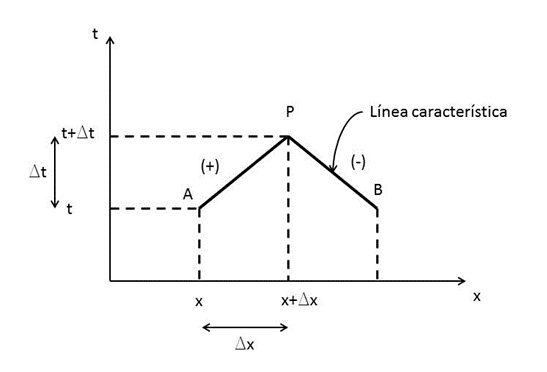
\includegraphics[width=0.8\linewidth]{figuras/fig21}
	\caption{Plano $(x,t)$ con la representación de las ecuaciones características (elaboración propia).}
	\label{fig:fig21}
\end{figure}

\begin{figure}
	\centering
	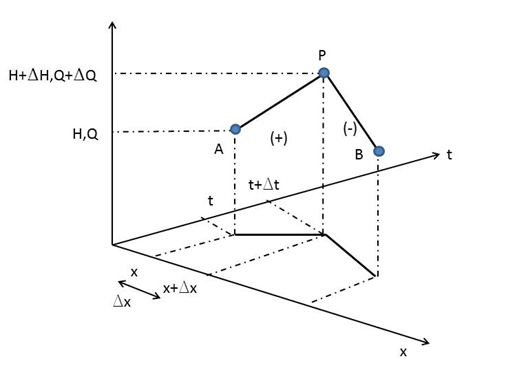
\includegraphics[width=0.8\linewidth]{figuras/fig22}
	\caption{Plano $H(x,t)$ o Q$(x,t)$ sobre las variables dependientes (elaboración propia).}
	\label{fig:fig22}
\end{figure}
\newpage

Entonces para la condición característica $(+)$ de $\dfrac{dx}{dt}=a$, se considera que $\dfrac{\Delta x}{\Delta t}\cong a$ y las variaciones de la función dependiente se evalúan como:
\begin{equation}
	dQ=Q_P-Q_A
\label{eq:dQ1}
\end{equation}

\begin{equation}
	dH=H_P-H_A
\label{eq:dQ2}
\end{equation}

y para la condición característica $(-)$ de $\dfrac{dx}{dt}=-a$, se considera que $\dfrac{\Delta x}{\Delta t}\cong -a$ y las variaciones de la función dependiente se evalúan como:
\begin{equation}
	dQ=Q_P-Q_B
	\label{eq:dQ3}
\end{equation}

\begin{equation}
	dH=H_P-H_B
\label{eq:dQ4}
\end{equation}

Para la característica positiva $(+)$ sustituyendo las ecuaciones \ref{eq:dQ1} y \ref{eq:dQ2} en \ref{eq:pos2} y además se considera una aproximación discreta para las derivadas temporales $\dfrac{dQ}{dt}\cong \dfrac{Q_P-Q_A}{\Delta t}$ y $\dfrac{dH}{dt} \cong \dfrac{H_P-H_A}{\Delta t}$, entonces:
\begin{equation}
	\dfrac{Q_P-Q_A}{\Delta t} + \dfrac{gA}{a}\dfrac{H_P-H_A}{\Delta t}+\dfrac{f|Q|Q}{2DA}=0
\end{equation}

En el caso la característica negativa $(-)$ se sustituyen las ecuaciones \ref{eq:dQ3} y \ref{eq:dQ4} en \ref{eq:pos4} y la aproximación discreta para las derivadas temporales $\dfrac{dQ}{dt}\cong \dfrac{Q_P-Q_B}{\Delta t}$ y $\dfrac{dH}{dt} \cong \dfrac{H_P-H_B}{\Delta t}$, 
\begin{equation}
	\dfrac{Q_P-Q_B}{\Delta t} + \dfrac{gA}{a}\dfrac{H_P-H_B}{\Delta t}+\dfrac{f|Q|Q}{2DA}=0
\end{equation}

Desarrollando:
\begin{equation}
	Q_P-Q_A\ +\frac{gA}{a}(H_P-H_A)+\dfrac{f|Q_A|Q_A\Delta t}{2DA}=0
\label{eq:pos5}
\end{equation}

\begin{equation}
	Q_P-Q_B\ +\frac{gA}{a}(H_P-H_B)+\dfrac{f|Q_B|Q_B\Delta t}{2DA}=0
	\label{eq:pos6}
\end{equation}

Nota: Para evaluar el término de fricción se considera la evaluación para el valor conocido, para la característica $(+\:)$ se toma $|Q_A|Q_A$ y para $(-\:)$ se considera $|Q_B|Q_B$.\bigskip
 
En un sentido más formal se puede considerar una condición intermedia, entonces para $(+)$ considerar $\delta Q^+=\dfrac{Q_A+Q_P}{2}$ y para $(-)$ considerar $\delta Q^-=\dfrac{Q_B+Q_P}{2}$, entonces se tiene que $|Q|Q=|\delta Q^+|\delta Q^+$ y $|Q|Q=|\delta Q^-|\delta Q^-$, respectivamente para las características $(+)$ y $(-)$.\bigskip

Desarrollando las ecuaciones \ref{eq:pos5} y \ref{eq:pos6} se tiene:
\begin{equation*}
	Q_P=-\dfrac{gA}{a}H_P+Q_A+\dfrac{gA}{a}H_A-\dfrac{f|Q_A|Q_A \Delta t}{2DA}
\end{equation*}

\begin{equation*}
	Q_P=\dfrac{gA}{a}H_P+Q_A-\dfrac{gA}{a}H_A-\dfrac{f|Q_B|Q_B \Delta t}{2DA}
\end{equation*}

o también,
\begin{equation}
	Q_P=C_\beta-C_\alpha H_P
\label{eq:qp1}
\end{equation}

\begin{equation}
	Q_P=C_\gamma-C_\alpha H_P
\label{eq:qp2}
\end{equation}

donde:
\begin{equation}
	C_\alpha=\dfrac{gA}{a}
\label{eq:qp3}
\end{equation}

\begin{equation}
	C_\beta=Q_A+C_\alpha H_A-\dfrac{f(|\frac{Q_A}{A}|,D,e)|Q_A|Q_A \Delta t}{2DA}
\label{eq:qp4}
\end{equation}

\begin{equation}
	C_\gamma=Q_B-C_\alpha H_B-\dfrac{f(\frac{Q_A}{A},D,e)|Q_B|Q_B \Delta t}{2DA}
\label{eq:qp5}
\end{equation}

Finalmente, la solución aproximada de las ecuaciones \ref{eq:pos5} y \ref{eq:pos6} se obtiene al resolver las ecuaciones algebraicas \ref{eq:qp1} y \ref{eq:qp2}, para lo cual se puede resolver en forma práctica, aplicando una suma término a término, entonces:
\begin{equation}
	{2Q}_P=C_\beta+C_\gamma+0
\end{equation}
o también,

\begin{equation}
	Q_P=\frac{C_\beta+C_\gamma}{2}
\label{eq:qp6}
\end{equation}

Con el resultado de la ecuación \ref{eq:qp6} (valores para $Q_P$ se pueden calcular con el valor de $H_P$ en la ecuación \ref{eq:qp1} o \ref{eq:qp2}.
\begin{equation}
	H_P=\frac{C_\beta-Q_P}{C_\alpha}
\end{equation}

\begin{equation}
	H_P=\frac{C_\gamma+Q_P}{C_\alpha}
\end{equation}

\subsection{Representación gráfica de la solución aproximada con MOC}
En forma esquemática el sistema de solución por el método de las características se puede observar en la Figura \ref{fig:fig23}
\begin{figure}[H]
	\centering
	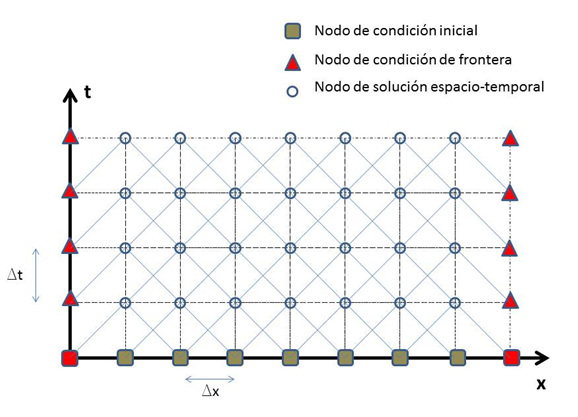
\includegraphics[width=0.7\linewidth]{fig23}
	\caption{Representación del plano $(x,t)$ discreto con las líneas características (elaboración propia)}
	\label{fig:fig23}
\end{figure}

\subsection{Notación para programación}
Sea el sistema de ecuaciones algebraicas:
\begin{equation}
	Q_P=C_\beta-C_\alpha H_P
\label{eq:qp7}
\end{equation}

\begin{equation}
	Q_P={C_\gamma+C}_\alpha H_P
\label{eq:qp8}
\end{equation}

Considerando que se tiene una malla espacio - temporal uniforme con intervalos constante $\Delta x$, $\Delta t$, que divide la 
región $\Omega(x,y)$, ver Figura \ref{fig:fig24} y permite establecer valores discretos de las variables dependiente, esto es:
\begin{equation}
	Q_j^n=Q(j\ \Delta x,\ n\ \Delta t)
\label{eq:qp9}
\end{equation}

\begin{equation}
	H_j^n=H(j\ \Delta x,\ n\ \Delta t)
\label{eq:qp10}
\end{equation}

Entonces el sistema \ref{eq:qp7} y \ref{eq:qp8}, se puede escribir como:
\begin{equation}
	Q_j^{n+1}={C_\beta}_j^n-C_\alpha H_j^{n+1}
\label{eq:qp11}
\end{equation}

\begin{equation}
	Q_j^{n+1}={C_\gamma}_j^n+C_\alpha H_j^{n+1}
\label{eq:qp12}
\end{equation}

Y las constantes en la representación espacial del plano de la \ref{fig:fig24}
\begin{equation}
	C_\alpha=\frac{gA}{a}
\label{eq:qp13}
\end{equation}

\begin{equation}
	{C_\beta}_j^n=Q_{j-1}^n+C_\alpha H_{j-1}^n-\dfrac{f|Q_{j-1}^n|Q_{j-1}^n \Delta t}{2DA}
\label{eq:qp14}
\end{equation}

\begin{equation}
	{C_\gamma}_j^n=Q_{j+1}^n-C_\alpha H_{j+1}^n-\dfrac{f|Q_{j+1}^n|Q_{j+1}^n \Delta t}{2DA}
\label{eq:qp15}
\end{equation}

La solución de la propagación temporal para $Q_j^{n+1}$, se obtiene como:
\begin{equation}
	Q_j^{n+1}=\dfrac{{C_\beta}_j^n+{C_\gamma}_j^n}{2}
\label{eq:qp16}
\end{equation}

Para calcular $H_j^{n+1}$, se pueden utilizar las expresiones:
\begin{equation}
	H_j^{n+1}=\dfrac{{C_\beta}_j^n-Q_j^{n+1}}{C_\alpha}
\label{eq:qp17}
\end{equation}

o también:
\begin{equation}
	H_j^{n+1}=\frac{{C_\gamma}_j^n-Q_j^{n+1}}{C_\alpha}
\label{eq:qp18}
\end{equation}

\begin{figure}[H]
	\centering
	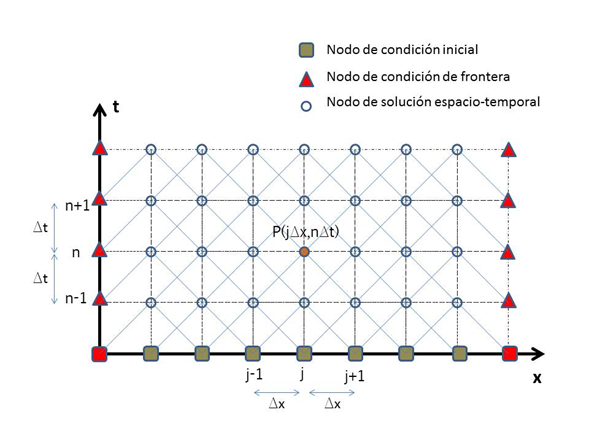
\includegraphics[width=0.8\linewidth]{figuras/fig24}
	\caption{Representación de la malla regular discreta sobre el dominio de solución $\Omega(x,y)$ (elaboración propia).}
	\label{fig:fig24}
\end{figure}

% **********************
\section{Condiciones de frontera y programa numérico}
\subsection{Distintas condiciones de frontera (válvula, depósito, bombas, etc.)}
El sistema de ecuaciones de cantidad de movimiento y conservación de masa, para el análisis de transitorios hidráulicos en una tubería a presión son:
\begin{equation}
	L(H,Q;x,t)=gA\dfrac{\partial H}{\partial t}+a^2\dfrac{\partial Q}{\partial x}=0
\label{eq:qp19}
\end{equation}

\begin{equation}
	M(H,Q;x,t)=\dfrac{\partial Q}{\partial t}+gA\dfrac{\partial H}{\partial x}+\dfrac{1}{A}\dfrac{f|Q|Q}{2D}=0
\label{eq:qp20}
\end{equation}

Donde x es la coordenada en el sentido horizontal y t el tiempo, como variables independientes; $H(x,t)$ y $Q(x,t)$, la carga hidráulica y el caudal respectivamente como variables dependientes; además $(x,t) \in \Omega=[0,L]\times[0,T]$ delimitan el espacio de solución; $L$ la longitud de la conducción; $T$, tiempo final de la solución; $a$, celeridad de onda del golpe de ariete, ecuación \ref{eq:acuad}; $A$ el área de la sección transversal de la tubería; $D$, diámetro de la tubería; $f$ el coeficiente de fricción de Darcy, y $g$ constante de la aceleración de la gravedad.
\begin{equation}
	a=\sqrt{\dfrac{K}{\rho\left(1+\frac{K}{E}\psi\right)}}
\label{eq:qp21}
\end{equation}

donde $\psi$ es un parámetro adimensional que depende de las propiedades elásticas del conducto; $E$, el módulo de elasticidad de Young; $K$ y $\rho$, son el módulo de elasticidad y la densidad del fluido, respectivamente.
\begin{equation*}
	\dfrac{1}{\sqrt f}=-2\log_{10}{\left(\dfrac{\dfrac{\varepsilon}{D}}{3.7}+\dfrac{2.51}{Re\sqrt f}\right)}
\end{equation*}
donde $\varepsilon$, rugosidad de la tubería; $Re=\frac{QD}{A\upsilon}$ número de Reynolds, y $\upsilon$ la viscosidad cinemática.

\begin{mdframed}[backgroundcolor=verdeclaro]
	\textbf{Nota}: Para el desarrollo de la condición inicial de un flujo en una tubería es necesario construir un algoritmo de cálculo de la fricción, considerando lo siguiente:\\
	sea el número de Reynolds,
	\begin{equation*}
		Re=\frac{VD}{\nu}
	\end{equation*} 
	donde $Re$, es el número adimensional de Reynolds (Panton, 2013); $V$, la velocidad media en una tubería, $D$, el diámetro, y $\nu$, la viscosidad cinemática.
	La pérdida por fricción en función de la longitud, diámetro y velocidad del fluido en una tubería se puede determinar con la ecuación Darcy-Wiesbach (Streeter y Wylie, 1976).
	\begin{equation*}
		h_f=f\dfrac{L}{D}\dfrac{V^2}{2g}
	\end{equation*}
	donde, $h_f$, es la pérdida por fricción, $L$, longitud de la tubería, $f$, factor de fricción.
	El modelo del factor de fricción, esta en función de número de Reynolds, entonces:\\
	Para $Re<2300$, se aplica la ecuación de Blasius:
	\begin{equation*}
		f=\dfrac{64}{Re}
	\end{equation*}
	Para $Re\geq2300$ se aplica la ecuación de Colebrook-White:
	\begin{equation*}
		\frac{1}{\sqrt f}=-2\log_{10}{\left(\frac{\dfrac{\varepsilon}{D}}{3.7}+\frac{2.51}{Re\sqrt f}\right)}
	\end{equation*} 
	\textbf{Tarea 2.} 
	Sea un embalse de 85 m de carga y tiene una tubería de descarga recta horizontal de 4.5 m de diámetro y con una longitud de 650 m. El material de la tubería es de acero al carbón, sin recubrimiento epóxico. Esta conducción tiene una rejilla y un codo de descarga de 45° a la salida.\bigskip
	\begin{itemize}
		\item Elaborar el diagrama de flujo para calcular el gasto de descarga.
		\item Elaborar el código en Matlab, Octave o Python para el cálculo y que pueda ser posible cambiar las condiciones de fricción, diámetro y longitud de la tubería.
		\item Determinar el gasto para descarga libre y con una rejilla al inicio de la conducción.
	\end{itemize}
	
	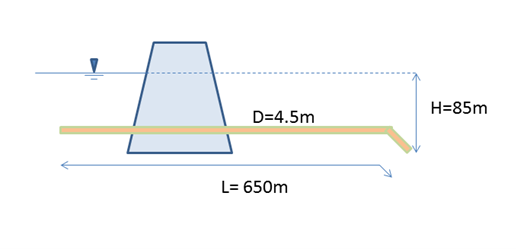
\includegraphics[width=0.7\linewidth]{figuras/tarea2}
	\label{fig:tarea2}\bigskip
	
	Ayuda: para esta tarea y las subsecuentes en el curso se recomienda, generar una función para el cálculo de la fricción en una tubería que resuelva las ecuaciones de Colebrook-White y Blasius. Para solucionar el problema es necesario aplicar la ecuación de la energía de Bernoulli y las condiciones de fricción, el algoritmo es no lineal pero tiene convergencia aplicando el método de punto fijo (Burden y Faires, 1985).
\end{mdframed}
El sistema de ecuaciones \ref{eq:qp19} y \ref{eq:qp20} constituye un problema bien planteado de valor inicial y de valores en la frontera, que está sujeto a las condiciones iniciales:
\begin{equation}
	H(x,0)=H_o(x)
\end{equation}

\begin{equation}
	Q(x,0)=Q_o(x)
\end{equation}

Las condiciones de frontera se definen para presión al inicio de la tubería y caudal en la descarga:
\begin{equation}
	H(0,t)=f(t) \hspace{1cm} ; \hspace{1cm} t>0
\label{eq:cf1}
\end{equation}

\begin{equation}
	Q(L,t)=g(t) \hspace{1cm} ; \hspace{1cm} t>0
\label{eq:cf2}
\end{equation}

El sistema \ref{eq:qp19} y \ref{eq:qp20} se ha discretizado aplicando el \underline{Método de las Características} y se tiene el siguiente sistema de ecuaciones algebraicas:
\begin{equation}
	Q_P=C_\beta-C_\alpha H_P
\label{eq:qp22}
\end{equation}

\begin{equation}
	Q_P={C_\gamma+C}_\alpha H_P
\label{eq:qp23}
\end{equation}

donde:
\begin{equation}
	C_\alpha=\dfrac{gA}{a}
\end{equation}

\begin{equation}
	C_\beta=Q_A+C_\alpha H_A-\dfrac{f|Q_A|Q_A \Delta t}{2DA}
\end{equation}

\begin{equation}
	C_\gamma=Q_B-C_\alpha H_B-\dfrac{f|Q_B|Q_B \Delta t}{2DA}
\end{equation}
Para implementación del código se definirán las condiciones de frontera específica.

\subsection{Nivel constante del embalse aguas arriba}
En esta condición de frontera se evalúa los efectos de cambios de energía cinética del movimiento del fluido en la tubería y las pérdidas locales, ver Figura \ref{fig:fig25}:
\clearpage
\begin{figure}[H]
	\centering
	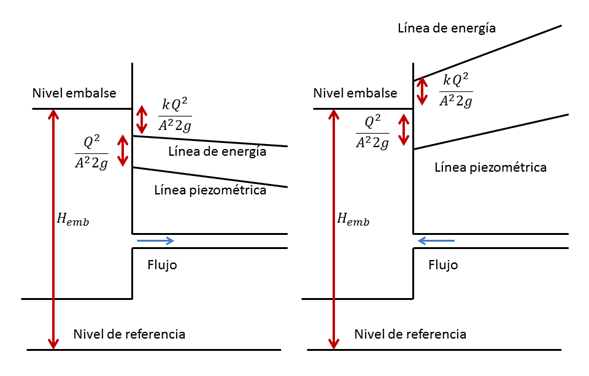
\includegraphics[width=0.9\linewidth]{figuras/fig25}
	\caption{Condición de frontera para nivel constante aguas arriba (elaboración propia).}
	\label{fig:fig25}
\end{figure}

La carga en el embalse se considera como:
\begin{equation}
	H_P=H_{emb}
\label{eq:qp24}
\end{equation}

donde $H_{emb}$ es la altura del agua dentro del embalse. Sustituyendo la ecuación \ref{eq:qp24} en la ecuación \ref{eq:qp23} (característica negativa debido a que la condición de movimiento de flujo se transmite de la tubería al embalse, Figura 2.26), entonces:
\begin{figure}[h]
	\centering
	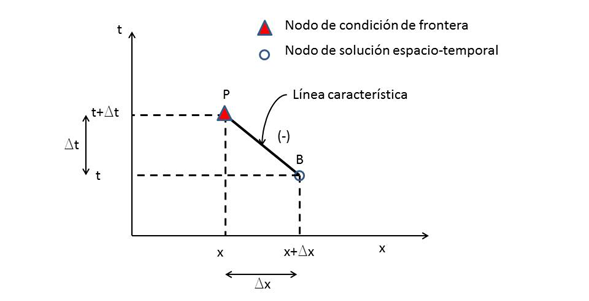
\includegraphics[width=1.0\linewidth]{figuras/fig26}
	\caption{Línea característica para evaluar el nodo en la frontera aguas arriba, en este caso $H_{emb}$ es conocido y falta calcular el gasto $Q_P$ (elaboración propia).}
	\label{fig:fig26}
\end{figure}

Si las pérdidas locales en la entrada de la tubería no son pequeñas (rejillas, deflectores, orientadores de flujo, etc.), estas pérdidas se evalúan como:
\begin{equation}
	h_e=\frac{kQ_P^2}{2gA^2}
\end{equation}

donde $k$ es la constante de pérdida local, considerando las cargas conforme a la Figura \ref{fig:fig26} se tiene:
\begin{equation*}
	H_P=H_{emb}-\frac{Q_P^2}{2gA^2}-\frac{kQ_P^2}{2gA^2}
\end{equation*}
o también:
\begin{equation}
	H_P=H_{emb}-(1+k)\dfrac{Q_P^2}{2gA^2}
\label{eq:qp25}	
\end{equation}

Despejando la variable de carga $H_P$ de la ecuación característica \ref{eq:qp8} se tiene:
\begin{equation}
	H_P=\dfrac{Q_P-C_\gamma}{C_\alpha}
\label{eq:qp26}
\end{equation}

Igualando \ref{eq:qp25} y \ref{eq:qp26} y desarrollando:
\begin{equation*}
	\frac{Q_P-C_\gamma}{C_\alpha}=H_{emb}-\left(1+k\right)\frac{Q_P^2}{2gA^2}
\end{equation*}

\begin{equation*}
	Q_P^2\frac{\left(1+k\right)}{2gA^2}+Q_P\frac{1}{C_\alpha}-\frac{C_\gamma}{C_\alpha}-H_{emb}=0
\end{equation*}

\begin{equation*}
	Q_P^2+Q_P\frac{2gA^2}{\left(1+k\right)C_\alpha}-\frac{2gA^2}{\left(1+k\right)}\left(\frac{C_\gamma}{C_\alpha}+H_{emb}\right)=0
\end{equation*}

\begin{equation*}
	Q_P^2+Q_P\frac{2gA^2}{\left(1+k\right)C_\alpha}-\frac{2gA^2}{\left(1+k\right)C_\alpha}\left(C_\gamma+C_\alpha H_{emb}\right)=0
\end{equation*}

Aplicando la solución de una ecuación polinomial de segundo grado, entonces:
\begin{equation*}
	Q_P=\dfrac{-\dfrac{2gA^2}{\left(1+k\right)C_\alpha}\pm\sqrt{\left(\dfrac{2gA^2}{\left(1+k\right)C_\alpha}\right)^2+4\dfrac{2gA^2}{\left(1+k\right)C_\alpha}\left(C_\gamma+C_\alpha H_{emb}\right)}}{2}
\end{equation*}

\begin{equation*}
	Q_P=-\frac{gA^2}{\left(1+k\right)C_\alpha}\pm\sqrt{\left(\frac{gA^2}{\left(1+k\right)C_\alpha}\right)^2+\frac{2gA^2}{\left(1+k\right)C_\alpha}\left(C_\gamma+C_\alpha H_{emb}\right)}
\end{equation*}

\begin{equation*}
	Q_P=-\frac{gA^2}{\left(1+k\right)C_\alpha}\pm\frac{gA^2}{\left(1+k\right)C_\alpha}\sqrt{1+\frac{2\left(1+k\right)C_\alpha}{gA^2}\left(C_\gamma+C_\alpha H_{emb}\right)}
\end{equation*}

\begin{equation*}
	Q_P=\frac{gA^2}{\left(1+k\right)C_\alpha}\left[-1\pm\sqrt{1+\frac{2\left(1+k\right)C_\alpha}{gA^2}\left(C_\gamma+C_\alpha H_{emb}\right)}\right]
\end{equation*}

o también:
\begin{equation}
	Q_P=\frac{1}{{2K}_1}\left[-1\pm\sqrt{1+{4K}_1\left(C_\gamma+C_\alpha H_{emb}\right)}\right]
\end{equation}

donde:
\begin{equation}
	K_1=\dfrac{\left(1+k\right)C_\alpha}{2gA^2}
\end{equation}

Nota: para una aplicación correcta en flujo reverso se debe considerar el valor del coeficiente de pérdida local como $k=k\ sgn(Q_B)$, esto es debido a que en el análisis a entrada del flujo no consideró $h_e=\dfrac{k\left|Q_P\right|Q_P}{2gA^2}$.

\begin{equation}
	K_1=\dfrac{[1+k \ sgn(QB)]C_\alpha}{2gA^2}
\end{equation}

\subsection{Condición de frontera nivel constante aguas abajo}
Nota: para este caso las condiciones de frontera definidas en \ref{eq:cf1} y \ref{eq:cf2} son invertidas, tal que:
\begin{equation}
	H(L,t)=f(t) \hspace{1cm} ; \hspace{1cm} t>0
	\label{eq:cf3}
\end{equation}

\begin{equation}
	Q(0,t)=g(t) \hspace{1cm} ; \hspace{1cm} t>0
	\label{eq:cf4}
\end{equation}

El esquema de la condición de frontera aguas abajo se puede ver en la Figura \ref{fig:fig27}.
\begin{figure}[H]
	\centering
	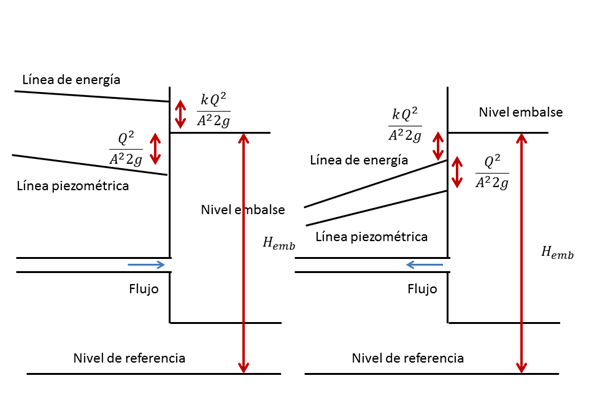
\includegraphics[width=0.9\linewidth]{figuras/fig27}
	\caption{Condición de frontera para nivel constante aguas abajo (elaboración propia).}
	\label{fig:fig27}
\end{figure}

Siguiendo un análisis similar a la condición de pérdida local a la salida se tiene que:
\begin{equation}
	H_P=H_{emb}-(1-k)\dfrac{Q_P^2}{2gA^2}
\end{equation}

y para el cálculo del gasto:
\begin{equation}
	Q_P=-\dfrac{1}{{2K}_1}\left[-1\pm\sqrt{1-{4K}_1(C_\beta-C_\alpha H_{emb})}\right]
\end{equation}

donde:
\begin{equation}
	K_2=\dfrac{(1-k)C_\alpha}{2gA^2}
\end{equation}

\subsection{Válvula aguas abajo}
\textbf{Opción I}\\
La condición flujo permanente que pasa por una válvula se puede expresar como:
\begin{equation}
	Q_o=(C_dA_v)_o\sqrt{2gH_o}
\label{eq:qp261}
\end{equation}

donde el subíndice $_o$ indica las variables en la condición permanente; $C_d$ coeficiente de descarga; $H_o$ carga aguas arriba de la válvula, y $A_v$ área hidráulica de la válvula. Construyendo la ecuación \ref{eq:qp261} en términos de las ecuaciones transitorias se tiene:
\begin{equation}
	Q_P=C_dA_v\sqrt{2gH_P}
\label{eq:qp27}
\end{equation}

Dividiendo \ref{eq:qp26} entre \ref{eq:qp27}:
\begin{equation*}
	\dfrac{Q_o}{Q_P}=\dfrac{(C_dA_v)_o}{C_dA_v}\sqrt{d\frac{H_o}{H_P}}
\end{equation*}

Considerando la variable auxiliar:
\begin{equation*}
	\tau=\dfrac{C_dA_v}{(C_dA_v)_o}
\end{equation*}

Entonces se tiene:
\begin{equation*}
	\dfrac{Q_o}{Q_P}=\dfrac{1}{\tau}\sqrt{\dfrac{H_o}{H_P}}
\end{equation*}

O también:
\begin{equation}
	Q_P^2=\dfrac{(Q_o\tau)^2}{H_o}H_P
\label{eq:qp28}
\end{equation}

En este caso se considera la característica positiva ya que se conoce la ley descarga, la cual es la variación de la apertura de la válvula, y la incógnita en la frontera aguas abajo es la presión, Figura \ref{fig:fig28}
 \begin{figure}[H]
	\centering
	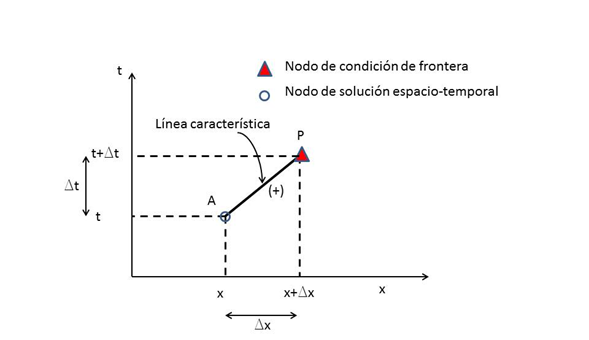
\includegraphics[width=1.0\linewidth]{figuras/fig28}
	\caption{Línea característica para evaluar el nodo en la frontera aguas abajo, en este caso $Q_P$ es conocido y falta calcular la presión $H_P$.}
	\label{fig:fig28}
\end{figure}

Sustituyendo la ecuación (2.91) e igualando con la ecuación \ref{eq:qp28} se tiene:
\begin{equation*}
	Q_P^2=\dfrac{(Q_o\tau)^2}{H_o}\frac{C_\beta-Q_P}{C_\alpha}
\end{equation*}

\begin{equation*}
	Q_P^2+Q_P\dfrac{(Q_o\tau)^2}{H_oC_\alpha}-\dfrac{\left(Q_o\tau\right)^2C_\beta}{H_oC_\alpha}=0
\end{equation*}

Considerando la variable auxiliar:
\begin{equation*}
	C_v=\dfrac{(Q_o\tau)^2}{H_oC_\alpha}
\end{equation*}

Entonces se tiene:
\begin{equation*}
	Q_P^2+Q_PC_v-C_vC_\beta=0
\end{equation*}

Y la solución se tiene para:
\begin{equation}
	Q_P=\dfrac{1}{2}\left[-C_v\pm\sqrt{C_v^2+4C_vC_\beta}\right]
\label{eq:qp29}
\end{equation}

Con el valor que se obtiene con la relación \ref{eq:qp29} se puede calcular $H_p$ con la ecuación (2.91).\bigskip

Nota: en la bibliografía existen otros tipos de condiciones de frontera para evaluar la inducción de un golpe de ariete sobre una conducción, en forma general estas son válidas si se respeta las condiciones definidas por las ecuaciones \ref{eq:qp26} y \ref{eq:qp27}.\bigskip

\textbf{Opción II}\\
Proponer una ley de cierre tal que $Q_p=Q_t(t)$ y con la ecuación (2.91) calcular el valor de $H_p$(característica positiva) entonces, la ley de cierre se define como:
\begin{equation}
	Q_t(t)=C_\beta-C_\alpha H_P
\label{eq:qp30}
\end{equation}

Y la carga en puntos de cierre se calcula con la siguiente expresión derivada (2.91):
\begin{equation}
	H_P=\frac{C_\beta-Q_t(t)}{C_\alpha}
\end{equation}

\section{Condición de estabilidad límite del esquema discreto}
En los estudios de convergencia numérica aplicando el teorema de Lax, y aplicando la expansión en serie de Taylor para el sistema discretizado, se considera por varios autores que la condición de Courant-Friedrichs-Lewy (Morton y Mayers, 2005) es suficiente si:
\begin{equation}
	\dfrac{\Delta t}{\Delta x}=\dfrac{1}{a}
\label{eq:qp31}
\end{equation}

\section{Programación MOC}
Para desarrollar el código numérico del esquema MOC en una tubería, en este caso se establecerá la condición siguiente:
\begin{itemize}
	\item Nivel del embalse constante.
	\item Válvula de operación agua abajo al final de la conducción.
	\item Política de cierre o apertura de la válvula conocida
\end{itemize}
Nota: Para condiciones diferentes a este caso de estudio no se analizarán en este curso, pero el estudiante cuenta con la formulación suficiente para generar un escenario distinto.\bigskip

Sea el sistema de ecuaciones para el análisis de transitorios hidráulicos en una tubería a presión son:
\begin{equation}
	L(H,Q;x,t)=gA\dfrac{\partial H}{\partial t}+a^2\dfrac{\partial Q}{\partial x}=0
\label{eq:qp32}
\end{equation}
	
\begin{equation}
	M(H,Q;x,t)=\dfrac{\partial Q}{\partial t}+gA\dfrac{\partial H}{\partial x}+\dfrac{1}{A}\dfrac{f|Q|Q}{2D}=0
\label{eq:qp33}
\end{equation}

Para discretizar el sistema continuo \ref{eq:qp32} y \ref{eq:qp33} en un esquema de numérico se considera una función continua $F:\Omega\rightarrow\mathbb{R}^2$, donde $\Omega(x,t)$ es el dominio espacio-temporal de solución y $\mathbb{R}$  el conjunto de los números reales. 
Si el espacio de solución $\Omega(x,t)$ es cubierto con una malla uniforme de espaciado $\Delta x$ para cualquier intervalo $\Delta t$, donde $\Delta x=\dfrac{L}{J}$,  $\Delta t=\dfrac{T}{N}$ y $J$ y $N$ son números enteros e indican la cantidad de intervalos computacionales de discretización espacial y temporal respectivamente, de forma que $\Omega\left(x_j,t_n\right)=\Omega(j\Delta x,n\Delta t)$ y el conjunto de puntos de los subíndices $j$ se agrupan en el vector $\mathbf{J}_\Omega$.\bigskip

En este espacio se tiene una variable discreta $f_j^n$ que se aproxima a $F(x_j,t_n)$ en cada punto $(x_j,t_n)$  del espacio $\Omega$.
\begin{figure}[H]
	\centering
	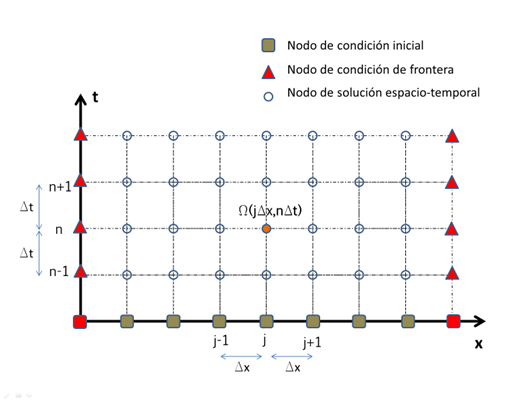
\includegraphics[width=0.8\linewidth]{figuras/fig29}
	\caption{Dominio de solución espacio-temporal (elaboración propia).}
	\label{fig:fig29}
\end{figure}

Entonces el sistema discreto de \ref{eq:mov2} y \ref{eq:masa22}  se puede escribir como:
\begin{equation}
	Q_j^{n+1}={C_\beta}_j^n-C_\alpha H_j^{n+1}
\end{equation}

\begin{equation}
	Q_j^{n+1}={C_\gamma}_j^n+C_\alpha H_j^{n+1}
\end{equation}

\begin{equation}
	C_\alpha=\frac{gA}{a}
\end{equation}

\begin{equation}
	{C_\beta}_j^n=Q_{j-1}^n+C_\alpha H_{j-1}^n-\dfrac{fQ_{j-1}^n Q_{j-1}^n\Delta t}{2DA}
\end{equation}

\begin{equation}
	{C_\gamma}_j^n=Q_{j+1}^n-C_\alpha H_{j+1}^n-\dfrac{fQ_{j+1}^nQ_{j+1}^n \Delta t}{2DA}
\end{equation}

Y la solución para $Q_j^{n+1}$, se representa como:
\begin{equation}
	Q_j^{n+1}=\dfrac{{C_\beta}_j^n+{C_\gamma}_j^n}{2}
\end{equation}

Para calcular $H_j^{n+1}$, se pueden utilizar las expresiones:
\begin{equation}
	H_j^{n+1}=\dfrac{{C_\beta}_j^n-Q_j^{n+1}}{C_\alpha}
\end{equation}

o:
\begin{equation}
	H_j^{n+1}=\dfrac{{C_\gamma}_j^n-Q_j^{n+1}}{C_\alpha}
\end{equation}

Procedimiento de cálculo:\\
Variables del problema del flujo en una tubería que se someterá a un cierre de la válvula.
\begin{mdframed}[backgroundcolor=azulpastel]
	\underline{Datos de la tubería:}\\
	Diámetro de la tubería (m), D = 0.3\\ 
	Rugosidad (m), $\varepsilon$ = 1x10$^{-5}$ \\
	Espesor de la tubería (pulgadas) = $\frac{1}{4}$\\ 
	Módulo de elasticidad de la tubería (GPa) = 200x10$^9$\\ 
	Relación de Poisson (adim.) = 0.3 \bigskip
	
	\underline{Datos de la conducción:}\\
	Pérdida local rejilla (adim.) = 0.5 \\
	Longitud de la conducción (m) = 26.67\\   
	Carga total del embalse (m) = 9.75'\\
	Altura de la descarga (m) = 0.0  \\
	Presión de la descarga (m) = 0.0  \\
	Aceleración de la gravedad (m/s$^2$) = 9.81 \\ 
	Coeficiente de descarga de la válvula = 0.65 \bigskip 
	
	\underline{Datos del fluido:}\\
	Módulo de elasticidad del agua (GPa) = 2.19x10$^9$  \\
	Viscosidad cinemática (m$^2$/s) = 1x10$^{-6}$ \\
	Densidad del fluido a 20°C (kg/m$^3$) = 999 \bigskip
	
	\underline{Tiempo de las condiciones de simulación:}\\
	Tiempo de inicio del cierre de la válvula (s); $T_inicio$ = 1.0\\  
	Tiempo total de simulación (s); $T_simulacion$ = 100.0 \bigskip
	
	\underline{Condición de frontera al final de la tubería (válvula):}\\
	Tiempo de cierre de la válvula (s): Tcierre = 2.0\\
	Política de cierre ($\tau$ vs t)\\
	Tiempo = [0.00 0.10 0.50 0.90 1.00]\\
	Tau = [1.00 0.95 0.50 0.05 0.00]\\
\end{mdframed}

\begin{enumerate}[a)]
	\item Determinar la condición de sujeción de la tubería ($\psi$), la celeridad de onda ($a$) y la condición de estabilidad límite $\Delta t$.
	\item Construcción de condición inicial:
		\begin{enumerate}[1.]
			\item Calcular el gasto de descarga de la tubería con fricción (tomar el algoritmo de la tarea no.2).
			\item Definir los valores de gasto y presión en la condición inicial (t=0):\\
			\begin{equation*}
				\begin{aligned}
					&Q_j^0=Qo \\
					&H_j^0=Ho(x_j)
				\end{aligned}
			\end{equation*}
		\end{enumerate}
	\item general la simulación para t>0:
		\begin{enumerate}[1.]
		\item Generar las variables ${C_{\beta}}_j^n$ y ${C_\gamma}_j^n$ (esta función debe tener implícito el cálculo de la fricción, tal como se aplicó en la tarea 2 y 3).
		\item Imponer la condición de frontera aguas abajo (válvula con la política de cierre) y aguas arriba (nivel del agua del embalse):\\
			\begin{equation*}
				\begin{aligned}
					&Q_J^{n+1}=g^{n+1} \\
					&H_J^{n+1}=\dfrac{{C_\beta}_j^n-Q_J^{n+1}}{C_\alpha}
				\end{aligned}
			\end{equation*}
		\item Considerar la condición de frontera aguas arriba (embalse con nivel constante).
			\begin{equation*}
				\begin{aligned}
				&K_1=\dfrac{[1+k_l \ sgn(Q_1^{n+1})]C_\alpha}{2gA^2} \\
				&Q_1^{n+1}=\dfrac{1}{{2K}_1}\left[-1\pm\sqrt{1+{4K}_1\left({C_\gamma}_1^n+C_\alpha H_{emb}\right)}\right] \\
				&H_1^{n+1}=H_{emb}-\left(1+k_l \ sgn(Q_1^{n+1}\right)\frac{\left(Q_1^{n+1}\right)^2}{2gA^2}
				\end{aligned}
			\end{equation*}
		\end{enumerate}
\end{enumerate}

\begin{figure}[H]
	\centering
	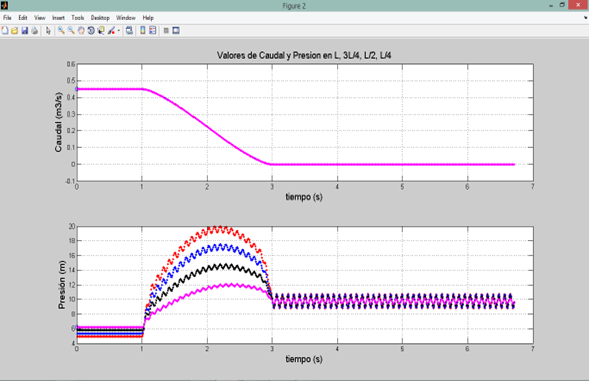
\includegraphics[width=0.9\linewidth]{figuras/fig30}
	\caption{Resultados de la modelación transitoria de una tubería sometida a un cierre de la válvula (elaboración propia).}
	\label{fig:fig30}
\end{figure}

\textbf{Tarea}\\
Elaborar un código numérico para simular el flujo transitorio de en tubería a presión, sometida al cierre o apertura de la válvula.\bigskip

Presentar los gráficos de variación de presión y caudal en diferentes puntos de la tubería y analizar la propagación de las ondas para diferentes tiempos de cierre.

\section{Referencias}
Burden, R., y Faires, J. (1985). \textit{Análisis numérico}. México D.F.: Grupo Editorial Iberoamericana.\bigskip

Chaudhry, M. (2014). \textit{Applied Hydraulic Transients}. (Third ed.). London: Springer-Verlag.\bigskip

Morton, K., y Mayers, D. (2005). \textit{Numerical solution of partial differential equations} (Second ed.). New York: Cambridge University Press.\bigskip

Panton, R. (2013). \textit{Incompressible flow} (4 ed.). Nueva York: John Wiley \& Sons Onc.\bigskip

Streeter, V., y Wylie, B. (1976). \textit{Mecánica de fluidos}. México: MacGraw-Hill.


\end{document}
